\documentclass[11pt]{article}
\usepackage[a4paper,margin=2.2cm]{geometry}
\usepackage[numbers]{natbib}
\usepackage{amsmath,amssymb,booktabs,graphicx,siunitx}
\usepackage{xr}
\externaldocument{main}
\renewcommand{\thesection}{S\arabic{section}}
\renewcommand{\thetable}{S\arabic{table}}
\renewcommand{\thefigure}{S\arabic{figure}}
\renewcommand{\theequation}{S\arabic{equation}}
\title{Supplementary Material for ``Anti-Windup under Amplitude and Slew-Rate Limits in Reverse-Acting Process Loops: An Implementation Study on an Exothermic CSTR''}
\author{Gabriel Marques de Andrade \and Elilton Rodrigues Edwards}
\date{}
\begin{document}
\maketitle
This supplement holds the analyses that are specific to the PID tunings of the test bed, and the full versions of tables condensed in the main text. Equation, table and figure numbers without the prefix S refer to the main text. Every table is generated by \texttt{experiments/build\_paper\_assets.py} from the released code; the CSV mirrors are in \texttt{results/jpc/}.

\section{Plant details}\label{supp:plant}
Moved from Section~\ref{sec:model} of the main text.

The Jacobian of Eqs.~\eqref{eq:cstr_ca}--\eqref{eq:cstr_tj} confirms it:
\begin{equation}
    \setlength{\arraycolsep}{5pt}
    \mathbf{A} = \begin{bmatrix}
        -19.923 & -0.0528 & 0 \\
        1892.33 & 3.282 & 1.0 \\
        0 & 5.000 & -10.00
    \end{bmatrix}, \quad
    \mathbf{B} = \begin{bmatrix} 0 \\ 0 \\ -2.416 \end{bmatrix},
    \label{eq:jacobian_matrices}
\end{equation}

Local stability does not guarantee global controllability. With the valve fully open, the jacket temperature cannot fall below
\begin{equation}
    T_{j,\min}(T) = \frac{u_{\max} T_{jf} + (UA/\rho_j C_{pj})\,T}{u_{\max} + UA/\rho_j C_{pj}} > T_{jf},
    \label{eq:tj_min_bound}
\end{equation}
so the heat that the reactor can reject is bounded by $Q_{r,\max}(T) = q \rho C_p (T - T_f) + UA\,(T - T_{j,\min}(T))$. Whenever a disturbance or a loss of heat-transfer capacity raises the required heat removal above $Q_{r,\max}$, no control law acting through this valve can hold the temperature; this bound is the physical controllability limit against which the PID loops are evaluated. The same balances solved backwards give the steady coolant flow that holds a temperature $T$,
\begin{equation}
    C_A^\star = \frac{(q/V)\,C_{Af}}{q/V + k(T)}, \quad
    T_j^\star = T - \frac{V\rho C_p}{UA}\!\left[\frac{q}{V}(T_f - T) + \frac{(-\Delta H)}{\rho C_p}\,k(T)\,C_A^\star\right], \quad
    u_{\mathrm{req}}(T) = \frac{UA\,(T - T_j^\star)}{\rho_j C_{pj}\,(T_j^\star - T_{jf})},
    \label{eq:u_req}
\end{equation}
with $k(T) = k_0\exp(-E/(R\,T))$. The setpoint is attainable at steady state only if $u_{\mathrm{req}} \le u_{\max}$; Section~\ref{subsec:sobol_results} uses $u_{\mathrm{req}}$ as the heat-removal demand of a perturbed plant. Conversely, a valve held at the upper stop settles the reactor at $T_\infty = T_{eq}(u_{\max})$, the steady temperature at full cooling ($377.94$~K for the nominal plant); $T_\infty$ is the offset equilibrium used in Section~\ref{subsec:clamping_rule}.

\section{Tuning study: design-model constraint, setpoint weighting and trade-offs}\label{supp:tuning}
These analyses concern the tunings themselves, not the anti-windup logic, and are not used by the conclusions of the main text. The two tunings below complete the test bed of the main text.
\begin{enumerate}
    \item \textbf{2-DOF AMIGO}: the AMIGO gains with setpoint weights $\beta = 0.5$, $\gamma = 0$ (Section~\ref{subsec:two_dof}), the use for which AMIGO is intended in servo tasks \cite{astrom2004revisiting}.
    \item \textbf{Optimal ITAE ($M_s^{\mathrm{FOPTD}} \le 1.6$)}: Nelder--Mead minimization of the ITAE of a $-2$~K step on the nonlinear plant and the benchmark valve, with the penalty $10^4\max(0, M_s - 1.6)^2$ and $M_s$ evaluated on the identified dead-time loop of Eq.~\eqref{eq:foptd}; the superscript records that the bound is imposed on the design model, not on the exact loop (Section~\ref{subsec:constraint_cost}). Evaluating $M_s$ on the delay-free Jacobian instead would return values close to one for almost any gain and silently disable the constraint. Because the simplex is local, it is started from a default guess and from every analytical tuning already inside the robust set (AMIGO, SIMC). The default start stops at a PI-like local optimum ($T_d = 0$, $\mathrm{ITAE} = 0.34$~K$\cdot$min$^2$); the analytical starts reach $0.20$--$0.21$~K$\cdot$min$^2$. The retained optimum has $M_s^{\mathrm{FOPTD}} = 1.60$: the constraint is active on the design model, and the derivative action is kept because it buys the phase margin that allows a higher proportional gain at the same $M_s$.
    \item \textbf{2-DOF Optimal ITAE}: the optimal gains with the setpoint weights fixed at $\beta = 0.5$, $\gamma = 0$. It is a 2-DOF \emph{variant}, not an optimized 2-DOF design; the joint optimization of gains and weights is reported in Section~\ref{subsec:constraint_cost}.
\end{enumerate}

\subsection{Two-degree-of-freedom setpoint weighting}
\label{subsec:two_dof}
A 2-DOF structure weights the reference in the proportional and derivative paths \cite{astrom2006pid}. To avoid a bias from absolute temperatures when $\beta < 1$, the weights act on deviations from $y_{ss} = 396.65$~K:
\begin{equation}
    e_p = \beta\,\Delta y_{sp} - \Delta y_{pv}, \qquad e_i = y_{sp} - y_{pv}, \qquad e_d = \gamma\,\Delta y_{sp} - \Delta y_{pv},
    \label{eq:two_dof}
\end{equation}
with $\Delta y = y - y_{ss}$, so that $P_k = K_p e_{p,k}$, the integrator is driven by $e_{i,k}$ and the derivative by $e_{d,k}$; $\gamma = 0$ recovers derivative on the measurement. Because $\beta$ and $\gamma$ act only on the reference path, the loop transfer function $L(s) = G_p(s)C(s)$, and therefore $M_s$ and the load response, are those of the 1-DOF controller with the same gains.

\subsection{Sensitivity peak and margins}
\label{subsec:sensitivity_theory}
Robustness is quantified by the sensitivity peak \cite{astrom2006pid, skogestad2005multivariable}
\begin{equation}
    M_s = \sup_{\omega \ge 0} \left|\frac{1}{1 + G_p(j\omega)C(j\omega)}\right|,
    \label{eq:sensitivity_func}
\end{equation}
evaluated with the exact delay $e^{-j\omega\theta}$ and $C(s) = K_p\,(1 + 1/(T_i s) + T_d s/(\tau_f s + 1))$. The bound $M_s \le 1.6$ guarantees a gain margin of at least $2.67$ and a phase margin of at least $36.4^\circ$ \cite{garpinger2014performance, padula2011tuning}. The FOPTD and the true plant agree at low frequency but diverge above the identification bandwidth: the delay adds phase lag without bound, whereas the phase of the relative-degree-two $G_{\text{true}}$ saturates. The FOPTD therefore overestimates the high-frequency lag, which makes $M_s$ conservative for loops whose peak lies at high frequency, while near crossover the comparison can go either way. Section~\ref{subsec:margins} evaluates both loops.

\subsection{Nominal step with the setpoint-weighted variants}
\begin{table*}[t]
\centering
\footnotesize
\caption{Nominal servo benchmark ($-2$~K setpoint step, noise-free) on the non-linear CSTR. FOPTD: $K=-0.1852$~K/(L/min), $\tau=0.6427$~min, $\theta=0.0935$~min. $M_s$ is evaluated on the dead-time FOPTD loop; TV includes the initial valve move from $\bar q_j$.}
\label{tab:classical_benchmark}
\resizebox{\ifdim\width>\textwidth\textwidth\else\width\fi}{!}{%
\begin{tabular}{lcccccccccc}
\toprule
Method & \(K_p\) & \(T_i\text{ (min)}\) & \(T_d\text{ (min)}\) & \(\beta\) & IAE & ITAE (K$\cdot$min$^2$) & TV (L/min) & \(M_p\text{ (\%)}\) & \(t_s\text{ (min)}\) & \(M_s\) \\
\midrule
Ziegler-Nichols & -44.56 & 0.187 & 0.047 & 1.0 & 0.940 & 0.316 & 81.9 & 22.6 & 1.38 & 4.14 \\
Cohen-Coon & -50.86 & 0.217 & 0.033 & 1.0 & 1.017 & 0.388 & 104.0 & 31.0 & 1.40 & 4.54 \\
Tyreus-Luyben & -28.10 & 0.779 & 0.056 & 1.0 & 0.917 & 0.336 & 48.8 & 0.0 & 1.64 & 2.32 \\
AMIGO & -17.79 & 0.327 & 0.045 & 1.0 & 0.925 & 0.308 & 40.4 & 9.7 & 1.44 & 1.45 \\
2-DOF AMIGO & -17.79 & 0.327 & 0.045 & 0.5 & 0.962 & 0.312 & 29.3 & 5.3 & 1.48 & 1.45 \\
Skogestad SIMC & -7.03 & 0.643 & 0.031 & 1.0 & 1.288 & 0.629 & 15.7 & 0.0 & 1.96 & 1.13 \\
Optimal ITAE ($M_s \leq 1.6$) & -23.55 & 0.465 & 0.032 & 1.0 & 0.827 & 0.204 & 48.6 & 2.2 & 0.94 & 1.60 \\
2-DOF Optimal ITAE & -23.55 & 0.465 & 0.032 & 0.5 & 1.084 & 0.424 & 25.0 & 0.0 & 1.62 & 1.60 \\
\bottomrule
\end{tabular}%
}
\end{table*}


With the directional rule of Eq.~\eqref{eq:clamping_antiwindup}, every tuning tracks the step. ZN and CC reach competitive errors ($\mathrm{IAE} = 0.940$ and $1.017$~K$\cdot$min) but with $M_s = 4.14$ and $4.54$, overshoots of $22.6\%$ and $31.0\%$ and $81.9$ and $104.0$~L/min of valve travel. Tyreus--Luyben gives $\mathrm{IAE} = 0.917$~K$\cdot$min without overshoot despite $M_s = 2.32$, and AMIGO ($M_s = 1.45$) gives $0.925$~K$\cdot$min with $9.7\%$ overshoot. Setpoint weighting reduces the AMIGO overshoot to $5.3\%$ and its travel from $40.4$ to $29.3$~L/min for a small increase in error ($0.962$~K$\cdot$min). SIMC ($M_s = 1.13$) is the most conservative tuning ($\mathrm{IAE} = 1.288$~K$\cdot$min, $\mathrm{TV} = 15.7$~L/min). Optimal ITAE, with its design-model constraint active ($M_s^{\mathrm{FOPTD}} = 1.60$), is the fastest loop of the benchmark ($\mathrm{IAE} = 0.827$~K$\cdot$min, $\mathrm{ITAE} = 0.204$~K$\cdot$min$^2$, settling in $0.94$~min with $2.2\%$ overshoot); its 2-DOF variant removes the overshoot and roughly halves the travel ($25.0$~L/min) at $\mathrm{IAE} = 1.084$~K$\cdot$min.

\subsection{Design-model versus plant robustness}
\label{subsec:margins}
Figure~\ref{fig:sensitivity_magnitude} shows $|S(j\omega)|$ on the FOPTD, and Table~\ref{tab:loop_margins} compares $M_s$ and the phase margin on the FOPTD and on the exact linearization of the plant with the half-sample hold delay $\Delta t/2$.

\begin{figure}[t]
    \centering
    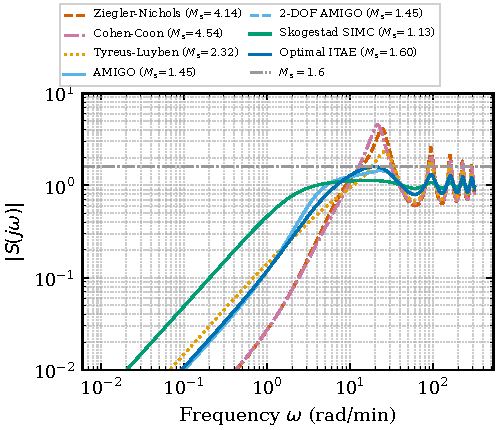
\includegraphics[width=0.92\columnwidth]{figures/fig_sensitivity_magnitude.pdf}
    \caption{Sensitivity magnitude $|S(j\omega)|$ on the identified dead-time FOPTD model. The 2-DOF variants share the loop of their 1-DOF counterparts.}
    \label{fig:sensitivity_magnitude}
\end{figure}

\begin{table*}[t]
\centering
\footnotesize
\caption{Sensitivity peak and phase margin of each PID loop on the identified FOPTD design model and on the exact Jacobian linearization of the CSTR at $\mathbf{x}_{ss}$ with the half-sample zero-order-hold delay $\Delta t/2 = 0.01$~min. Valve saturation and slew-rate limits are not part of either linear loop.}
\label{tab:loop_margins}
\resizebox{\ifdim\width>\textwidth\textwidth\else\width\fi}{!}{%
\begin{tabular}{lcccc}
\toprule
Method & \(M_s\) (FOPTD) & PM (FOPTD, \(^\circ\)) & \(M_s\) (lin.) & PM (lin., \(^\circ\)) \\
\midrule
Ziegler-Nichols & 4.14 & 36.6 & 1.57 & 38.4 \\
Cohen-Coon & 4.54 & 25.3 & 1.75 & 35.1 \\
Tyreus-Luyben & 2.32 & 72.3 & 1.15 & 71.1 \\
AMIGO & 1.45 & 59.3 & 1.26 & 53.9 \\
Skogestad SIMC & 1.13 & 81.7 & 1.11 & 78.7 \\
Optimal ITAE ($M_s^{\mathrm{FOPTD}} \leq 1.6$) & 1.60 & 61.1 & 1.31 & 57.1 \\
\bottomrule
\end{tabular}%
}
\end{table*}


The sensitivity peak on the linearized plant is lower than on the FOPTD for every tuning, and strongly so for the high-gain rules (ZN: $4.14 \rightarrow 1.57$, CC: $4.54 \rightarrow 1.75$, TL: $2.32 \rightarrow 1.15$). Their peaks lie at high frequency, where the FOPTD delay keeps adding phase lag that the relative-degree-two plant of Eq.~\eqref{eq:g_true_exact} does not have; together with the rate limit, which clips the initial proportional kick into a bounded ramp, this explains why ZN and CC do not oscillate on the noise-free step. The phase margin, set near crossover, behaves differently: for the moderate-bandwidth designs the FOPTD is slightly optimistic (AMIGO: $59.3^\circ$ versus $53.9^\circ$, Optimal ITAE: $61.1^\circ$ versus $57.1^\circ$, SIMC: $81.7^\circ$ versus $78.7^\circ$), whereas for ZN and CC it is pessimistic ($36.6^\circ$ versus $38.4^\circ$ and $25.3^\circ$ versus $35.1^\circ$). The $M_s \le 1.6$ constraint imposed on the FOPTD is thus a conservative proxy for the peak sensitivity of the real loop (Section~\ref{subsec:constraint_cost} measures what that conservatism costs), but the designer should allow for a loss of up to $5.4^\circ$ of phase margin at crossover. Neither linear loop contains the rate limit, which adds an amplitude-dependent phase lag during large moves; the table describes small-signal behaviour.

\begin{table*}[t]
\centering
\footnotesize
\caption{Plant-exact robustness of the six feedback loops on the Jacobian linearization at $\mathbf{x}_{ss}$ with the half-sample zero-order-hold delay, and the high-frequency controller gain that maps measurement noise into valve movement.}
\label{tab:exact_robustness}
\resizebox{\ifdim\width>\textwidth\textwidth\else\width\fi}{!}{%
\begin{tabular}{lccccc}
\toprule
Method & \(M_s\) (FOPTD) & \(\|S\|_\infty\) (lin.) & \(\|T\|_\infty\) (lin.) & \(\|CS\|_\infty\) (L/min/K) & \(K_{\mathrm{hf}}=|K_p|(1+N)\) (L/min/K) \\
\midrule
Ziegler-Nichols & 4.14 & 1.57 & 1.66 & 490.1 & 490.2 \\
Cohen-Coon & 4.54 & 1.75 & 1.72 & 559.2 & 559.5 \\
Tyreus-Luyben & 2.32 & 1.15 & 1.00 & 309.0 & 309.1 \\
AMIGO & 1.45 & 1.26 & 1.22 & 195.6 & 195.7 \\
Skogestad SIMC & 1.13 & 1.11 & 1.00 & 77.3 & 77.4 \\
Optimal ITAE ($M_s^{\mathrm{FOPTD}} \leq 1.6$) & 1.60 & 1.31 & 1.11 & 258.9 & 259.0 \\
\bottomrule
\end{tabular}%
}
\end{table*}


The sensitivity peak does not explain the noise behaviour of the empirical rules, because on the exact linearization their peaks are only $\|S\|_\infty = 1.57$ (ZN) and $1.75$ (CC); the values of $4.14$ and $4.54$ on the design model largely reflect the apparent delay of the FOPTD. What does distinguish the loops is the gain from measurement noise to the valve command, $CS = C/(1+L)$ (Table~\ref{tab:exact_robustness}). At high frequency $S \to 1$ and $CS \to C$, so $\|CS\|_\infty$ is attained on the plateau of the filtered PID, $K_{\mathrm{hf}} = |K_p|(1+N)$, and equals it to within $0.3$~L/min/K for all six loops: $490.1$ (ZN), $559.2$ (CC), $309.0$ (TL), $195.6$ (AMIGO), $258.9$ (Optimal ITAE) and $77.3$ (SIMC) L/min/K. ZN and CC therefore convert measurement noise into valve movement with $6$ to $7$ times the gain of SIMC, even though their loops are not close to instability.

\subsection{Cost of imposing the sensitivity bound on the design model}
\label{subsec:constraint_cost}
The Optimal ITAE tuning bounds $M_s$ on the identified dead-time model, whose apparent delay overstates the high-frequency lag; on the exact linearization the same gains have $M_s^{\mathrm{lin}} = 1.31$ and a phase margin of $57.1^\circ$ (Table~\ref{tab:constraint_cost}). To measure what the proxy costs, the optimization was repeated with $M_s^{\mathrm{lin}} \le 1.6$ imposed on the exact Jacobian loop with the half-sample zero-order hold, with the same objective, valve and multi-start (started from the default guess and from every analytical tuning inside the exact robust set, then restarted once from the winner).

\begin{table*}[t]
\centering
\footnotesize
\caption{Cost of the design-model constraint. Each tuning minimizes the ITAE of the $-2$~K step ($6$~min) subject to $M_s \le 1.6$ evaluated on the dead-time FOPTD ($M_s^{\mathrm{FOPTD}}$) or on the exact Jacobian loop with the half-sample zero-order hold ($M_s^{\mathrm{lin}}$); ``joint'' rows optimize $(K_p, T_i, T_d, \beta, \gamma)$ together, the 2-DOF row with $\beta = 0.5$ is the fixed-weight variant ($\beta = 0.5$, $\gamma = 0$) of Fig.~\ref{fig:classical_benchmark}. ITAE in K$\cdot$min$^2$, IAE in K$\cdot$min, TV in L/min, $K_{\mathrm{hf}}$ in (L/min)/K, PM at the highest gain crossover.}
\label{tab:constraint_cost}
\resizebox{\ifdim\width>\textwidth\textwidth\else\width\fi}{!}{%
\begin{tabular}{lccccccccccccccc}
\toprule
Tuning & \(K_p\) & \(T_i\) (min) & \(T_d\) (min) & \(\beta\) & \(\gamma\) & \(M_s^{\mathrm{FOPTD}}\) & \(M_s^{\mathrm{lin}}\) & PM$^{\mathrm{lin}}$ ($^\circ$) & \(K_{\mathrm{hf}}\) & IAE & ITAE & \(M_p\) (\%) & TV & ITAE $-5$ K & ITAE $+5$ K \\
\midrule
Optimal ITAE ($M_s^{\mathrm{FOPTD}} \leq 1.6$) & -23.55 & 0.465 & 0.032 & 1.00 & 0.00 & 1.60 & 1.31 & 57.1 & 259 & 0.827 & 0.204 & 2.2 & 48.6 & 1.292 & 1.200 \\
2-DOF Optimal ITAE & -23.55 & 0.465 & 0.032 & 0.50 & 0.00 & 1.60 & 1.31 & 57.1 & 259 & 1.084 & 0.424 & 0.0 & 25.0 & 1.756 & 1.564 \\
Joint 2-DOF ITAE ($M_s^{\mathrm{FOPTD}} \leq 1.6$) & -23.55 & 0.464 & 0.032 & 1.00 & 0.00 & 1.60 & 1.31 & 57.1 & 259 & 0.827 & 0.204 & 2.2 & 48.6 & 1.289 & 1.197 \\
Optimal ITAE ($M_s^{\mathrm{lin}} \leq 1.6$) & -41.41 & 0.597 & 0.093 & 1.00 & 0.00 & 13.86 & 1.20 & 75.5 & 456 & 0.799 & 0.181 & 0.7 & 59.6 & 1.322 & 1.239 \\
Joint 2-DOF ITAE ($M_s^{\mathrm{lin}} \leq 1.6$) & -46.23 & 0.558 & 0.099 & 0.98 & 0.09 & 12.95 & 1.24 & 74.4 & 508 & 0.799 & 0.181 & 0.8 & 60.7 & 1.307 & 1.257 \\
\bottomrule
\end{tabular}%
}
\end{table*}


The exact-loop optimum is interior: it stops at $M_s^{\mathrm{lin}} = 1.20$ ($\mathrm{PM} = 75.5^\circ$), so the exact bound is not active and it is the valve, not robustness, that caps the speed of the loop. Relaxing the design model to the exact loop lowers the design ITAE from $0.204$ to $0.181$~K$\cdot$min$^2$ ($-11.3\%$) and the IAE from $0.827$ to $0.799$~K$\cdot$min ($-3.4\%$), with overshoot $0.7\%$, at the price of a $1.76$ times higher proportional gain: the high-frequency gain rises from $259$ to $456$~L/min/K ($+76\%$) and the valve travel from $48.6$ to $59.6$~L/min ($+22.6\%$). The gain does not carry over outside the design step: the ITAE on the $-5$ and $+5$~K steps is $2.3\%$ and $3.3\%$ \emph{higher} than that of the FOPTD-bounded tuning (Table~\ref{tab:out_of_sample}). The 11\% ITAE of the exact-loop optimum is therefore an in-sample gain with no counterpart outside the design step, and it is paid for in noise gain: the FOPTD-bounded tuning has $43\%$ lower high-frequency gain ($259$ against $456$~L/min/K). The phrase ``fastest robust PID'' is not used for either tuning, because the speed of the first is capped by the proxy and that of the second by the rate limit.

Optimizing the setpoint weights jointly with the gains returns the 1-DOF controller. Under the FOPTD bound the optimum has $\beta = 1.00$ and $\gamma = 0.00$ with the same ITAE ($0.204$); under the exact bound $\beta = 0.98$ and $\gamma = 0.09$ with the same ITAE ($0.181$) and a $12\%$ higher proportional gain. Setpoint weighting does not help a tracking objective that has no cost on the valve; the fixed weight $\beta = 0.5$ of the 2-DOF variant is a deliberate trade of $+31.1\%$ IAE for $-48.6\%$ valve travel and no overshoot, not an optimum, and it is called a variant, not ``optimal'', in the remainder of the paper.

\paragraph{Model error.} The margin of the exact-loop optimum is also more exposed to model error (Table~\ref{tab:model_error}). The test is like-for-like: the same exact plant and the same $18$ perturbations for every tuning (loop gain and all plant time constants, $\tau$ included, scaled by $0.8$, $1$ and $1.2$, and an extra delay of $0$ or $0.2\,\theta_{\mathrm{FOPTD}}$), with the stability of every corner decided from the closed-loop polynomial and $M_s$ taken over the stable corners only. No tuning has an unstable corner. The worst $M_s$ is $1.63$ for the FOPTD-bounded optimum ($1.31$ nominal), $2.06$ for the exact-loop optimum ($1.20$ nominal), $2.84$ and $3.42$ for ZN and CC, $1.42$ for TL, $1.59$ for AMIGO and $1.20$ for SIMC: its peak rises by $72\%$ over the nominal value against $24\%$ for the FOPTD-bounded one, but it stays stable at every corner and better than ZN and CC. Deadband (Section~\ref{subsec:ablation}) was simulated for the anti-windup policies and not for $M_s$; stiction was not simulated.

\begin{table*}[t]
\centering
\footnotesize
\caption{Sensitivity peak under model error: on the FOPTD, the largest $M_s$ over the $27$ corners of $K$, $\tau$, $\theta$ scaled by $0.8$, $1$, $1.2$; on the exact loop, the largest $M_s$ with the loop gain scaled by $0.8$ or $1.2$ and an extra delay of $0.2\,\theta_{\mathrm{FOPTD}}$. Deadband and stiction are not modelled.}
\label{tab:model_error}
\resizebox{\ifdim\width>\textwidth\textwidth\else\width\fi}{!}{%
\begin{tabular}{lcccc}
\toprule
Tuning & \(M_s^{\mathrm{FOPTD}}\) nominal & worst of $27$ corners & \(M_s^{\mathrm{lin}}\) nominal & worst ($K\pm20\%$, $+0.2\theta$) \\
\midrule
Optimal ITAE ($M_s^{\mathrm{FOPTD}} \leq 1.6$) & 1.60 & 2.74 & 1.31 & 1.56 \\
Optimal ITAE ($M_s^{\mathrm{lin}} \leq 1.6$) & 13.86 & 151.77 & 1.20 & 1.60 \\
AMIGO & 1.45 & 2.02 & 1.26 & 1.44 \\
Skogestad SIMC & 1.13 & 1.25 & 1.11 & 1.18 \\
\bottomrule
\end{tabular}%
}
\end{table*}


\subsection{Out-of-sample setpoint steps}
\label{subsec:oos}
The Optimal ITAE gains were fitted on the $-2$~K step, so their advantage in Table~\ref{tab:classical_benchmark} is in-sample. Table~\ref{tab:out_of_sample} evaluates every tuning on steps of $-5$, $-1$, $+1$, $+2$ and $+5$~K with the same valve, anti-windup and horizon ($10$~min; the optimizer used $6$~min).

\begin{table*}[t]
\centering
\footnotesize
\caption{ITAE (K$\cdot$min$^2$) of every tuning on setpoint steps of different size and sign. The Optimal ITAE gains were fitted on the $-2$~K step only (in-sample column); all other columns are out-of-sample. Same valve, directional anti-windup and $10$~min horizon.}
\label{tab:out_of_sample}
\resizebox{\ifdim\width>\textwidth\textwidth\else\width\fi}{!}{%
\begin{tabular}{lcccccc}
\toprule
Method & -5 K & -2 K & -1 K & +1 K & +2 K & +5 K \\
\midrule
Ziegler-Nichols & 1.413 & 0.316 & 0.084 & 0.105 & 0.345 & 1.985 \\
Cohen-Coon & 1.571 & 0.388 & 0.111 & 0.131 & 0.465 & 3.373 \\
Tyreus-Luyben & 1.876 & 0.336 & 0.092 & 0.091 & 0.327 & 1.716 \\
AMIGO & 1.389 & 0.308 & 0.122 & 0.108 & 0.250 & 0.969 \\
2-DOF AMIGO & 1.605 & 0.312 & 0.118 & 0.105 & 0.260 & 1.136 \\
Skogestad SIMC & 2.961 & 0.629 & 0.229 & 0.204 & 0.499 & 1.890 \\
Optimal ITAE ($M_s \leq 1.6$) & 1.292 & 0.204 & 0.065 & 0.063 & 0.192 & 1.200 \\
2-DOF Optimal ITAE & 1.756 & 0.424 & 0.154 & 0.153 & 0.414 & 1.564 \\
Rank of Optimal ITAE (1 = best) & 1 & 1 & 1 & 1 & 1 & 3 \\
\bottomrule
\end{tabular}%
}
\end{table*}


The optimum generalizes to steps of both signs up to $5$~K in the cooling direction and $2$~K in the heating direction: among the eight benchmark tunings it has the lowest ITAE at $-5$ ($1.292$), $-1$ ($0.065$), $+1$ ($0.063$) and $+2$~K ($0.192$). At $+5$~K it ranks third ($1.200$), behind AMIGO ($0.969$) and 2-DOF AMIGO ($1.136$), so the in-sample optimum is not uniformly optimal for the largest heating step. The tunings that were re-optimized in Section~\ref{subsec:constraint_cost} do not change the picture: the exact-loop optimum wins in-sample ($0.181$) and at $+1$~K ($0.062$) but loses to the FOPTD-bounded one at $-5$, $-1$, $+2$ and $+5$~K, and the jointly optimized 2-DOF designs coincide with their 1-DOF counterparts to within $0.02$~K$\cdot$min$^2$.

\subsection{Tracking error versus valve travel}
\label{subsec:pareto_results}
The trade-off between tracking accuracy and actuator wear was mapped by sweeping the SIMC closed-loop time constant over $\tau_c \in [0.015, 2.5]$~min ($45$ logarithmically spaced points) and by minimizing $\lambda\,\mathrm{IAE}/\mathrm{IAE}_0 + (1 - \lambda)\,\mathrm{TV}/\mathrm{TV}_0$ for $\lambda \in [0.05, 0.95]$ (Fig.~\ref{fig:pareto_iae_tv}, Table~\ref{tab:pareto_tradeoff}).

\begin{figure*}[t]
    \centering
    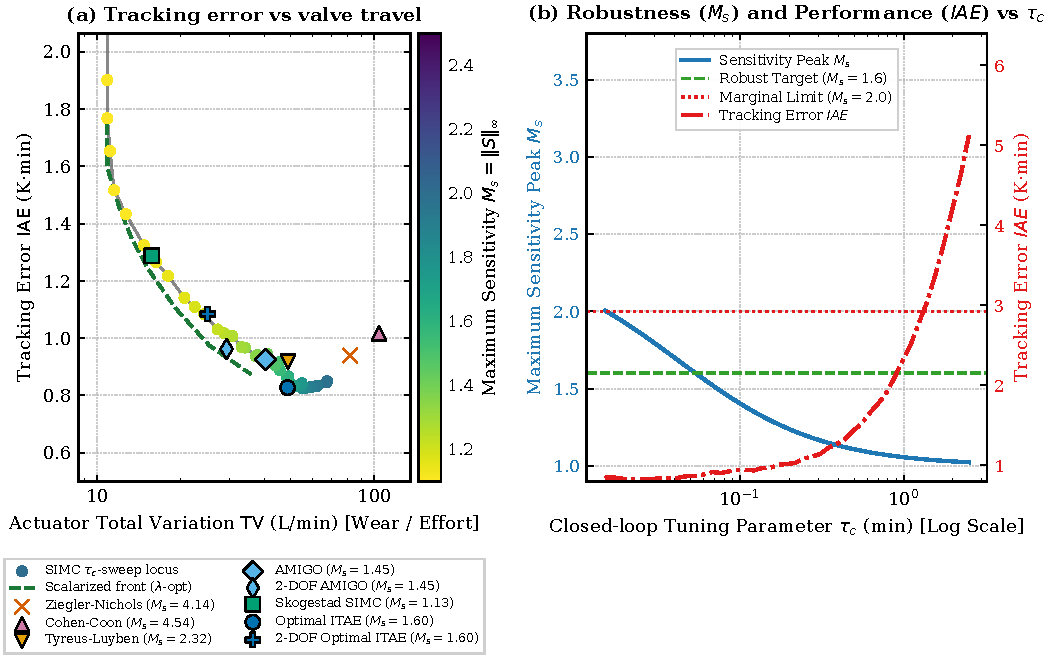
\includegraphics[width=0.92\textwidth]{figures/fig4_pareto_iae_tv.pdf}
    \caption{(a) SIMC $\tau_c$-sweep locus (colour: $M_s$), scalarized optimal front ($\lambda$-opt) and the discrete tunings in the $(\mathrm{TV}, \mathrm{IAE})$ plane (logarithmic TV axis); (b) $M_s$ and IAE as functions of $\tau_c$.}
    \label{fig:pareto_iae_tv}
\end{figure*}

\begin{table*}[t]
\centering
\footnotesize
\caption{Trade-off along the SIMC $\tau_c$ locus and for the discrete rules: robustness ($M_s$), tracking error and actuator effort (TV); the locus is a one-parameter family, not a Pareto frontier.}
\label{tab:pareto_tradeoff}
\resizebox{\ifdim\width>\textwidth\textwidth\else\width\fi}{!}{%
\begin{tabular}{lccccccc}
\toprule
Strategy & $K_{p}$ & $T_{i}$ (min) & $T_{d}$ (min) & $M_{s}$ & IAE (K$\cdot$min) & TV (L/min) & $M_{p}$ (\%) \\
\midrule
SIMC ($\tau_c=0.03$) & -28.08 & 0.49 & 0.03 & 1.79 & 0.83 & 54.2 & 0.3 \\
SIMC ($\tau_c=0.10$) & -18.28 & 0.64 & 0.03 & 1.41 & 0.95 & 41.0 & 0.0 \\
SIMC ($\tau_c=0.24$) & -10.27 & 0.64 & 0.03 & 1.20 & 1.08 & 24.3 & 0.0 \\
SIMC ($\tau_c=0.39$) & -7.19 & 0.64 & 0.03 & 1.13 & 1.27 & 16.3 & 0.0 \\
SIMC ($\tau_c=0.78$) & -3.97 & 0.64 & 0.03 & 1.07 & 1.90 & 10.9 & 0.0 \\
SIMC ($\tau_c=1.57$) & -2.09 & 0.64 & 0.03 & 1.04 & 3.40 & 10.9 & 0.0 \\
Ziegler-Nichols & -44.56 & 0.19 & 0.05 & 4.14 & 0.94 & 81.9 & 22.6 \\
Cohen-Coon & -50.86 & 0.22 & 0.03 & 4.54 & 1.02 & 104.0 & 31.0 \\
Tyreus-Luyben & -28.10 & 0.78 & 0.06 & 2.32 & 0.92 & 48.8 & 0.0 \\
AMIGO & -17.79 & 0.33 & 0.04 & 1.45 & 0.93 & 40.4 & 9.7 \\
2-DOF AMIGO & -17.79 & 0.33 & 0.04 & 1.45 & 0.96 & 29.3 & 5.3 \\
Skogestad SIMC & -7.03 & 0.64 & 0.03 & 1.13 & 1.29 & 15.7 & 0.0 \\
Optimal ITAE ($M_s^{\mathrm{FOPTD}} \leq 1.6$) & -23.55 & 0.47 & 0.03 & 1.60 & 0.83 & 48.6 & 2.2 \\
2-DOF Optimal ITAE & -23.55 & 0.47 & 0.03 & 1.60 & 1.08 & 25.0 & 0.0 \\
\bottomrule
\end{tabular}%
}
\end{table*}


Along the SIMC locus the error decreases monotonically as $\tau_c$ shrinks ($1.90$, $1.27$, $1.08$, $0.95$ and $0.83$~K$\cdot$min for $\tau_c = 0.78$, $0.39$, $0.24$, $0.10$ and $0.03$~min) while $M_s$ rises from $1.07$ to $1.79$ and the travel from $10.9$ to $54.2$~L/min: speed is bought with robustness, and with a correct anti-windup the rate limit creates no interior optimum. For $\tau_c \ge 0.78$~min the travel reaches its floor of $10.9$~L/min, the net change of steady-state coolant flow required by the new setpoint. The scalarized front lies slightly below the SIMC locus, so a free PID improves on SIMC by a small margin at equal travel. SIMC, 2-DOF AMIGO and 2-DOF Optimal ITAE lie close to the front; AMIGO, TL and Optimal ITAE sit on its high-gain branch; ZN and CC are dominated, with more error and more travel than Optimal ITAE at $2.6$ to $2.8$ times its design $M_s$.

\section{Anti-windup: full tables and discussion}\label{supp:aw}
Full versions of the results condensed in Section~\ref{subsec:ablation} of the main text.

\begin{table*}[t]
\centering
\footnotesize
\caption{Windup mechanism of the empirical rules on the $-2$~K step: lowest reactor temperature, time with the valve at its upper stop, final tracking error and largest command--valve discrepancy $\max|u_{\text{raw}}-u_{\text{act}}|$.}
\label{tab:antiwindup_mechanism}
\resizebox{\ifdim\width>\textwidth\textwidth\else\width\fi}{!}{%
\begin{tabular}{lccccc}
\toprule
Method & Anti-windup & \(T_{\min}\) (K) & Time at \(u_{\max}\) (min) & \(T(t_f)-T_{sp}\) (K) & \(\max|u_{\mathrm{raw}}-u_{\mathrm{act}}|\) (L/min) \\
\midrule
Ziegler-Nichols & None & 382.0 & 0.00 & +17.15 & 7775 \\
Ziegler-Nichols & Sign-blind amp. & 377.8 & 3.86 & -16.72 & 4474 \\
Ziegler-Nichols & Amp.+rate direct. (Eq.~13) & 394.2 & 0.00 & +0.00 & 92 \\
Cohen-Coon & None & 382.8 & 0.00 & +8.52 & 8022 \\
Cohen-Coon & Sign-blind amp. & 377.8 & 4.06 & -16.72 & 3540 \\
Cohen-Coon & Amp.+rate direct. (Eq.~13) & 394.0 & 0.00 & -0.00 & 105 \\
\bottomrule
\end{tabular}%
}
\end{table*}


\paragraph{Why sign-blind clamping locks the valve at full cooling.} For ZN and CC the sign-blind rule is not merely ineffective, it is worse than no anti-windup (IAE $104.12$ and $102.67$ against $91.11$ and $87.37$~K$\cdot$min), and it fails in two steps. First, the slew limit lets the command run away from the valve position (by up to $4474$~L/min for ZN) while the valve is far from its stops. The condition ``$u_{\text{raw}} \ge u_{\max}$ and $e_k > 0$'' was written for a direct-acting loop. With $K_p < 0$, an overheated reactor ($T > T_{sp}$, $e_k < 0$) pushes the command \emph{up} towards $u_{\max}$; the product of the conditions is never true in that situation, so the integrator is never frozen when it should be and it winds up (the amplitude-only rule also misses the slew-rate cut). Second, the wound-up command drives the reactor below the setpoint ($e_k > 0$) while $u_{\text{raw}} \gg u_{\max}$ (the discrepancy is $3.5$--$4.5\times 10^{3}$~L/min); now both conditions hold and the rule \emph{freezes} the integrator, precisely when it must unwind. The valve reaches $u_{\max} = 300$~L/min at $t = 6.16$~min (ZN) and stays there until $t_f$, $3.86$ and $4.06$~min at the upper stop in Table~\ref{tab:antiwindup_mechanism}, and the reactor settles at the open-loop steady state of $q_j = 300$~L/min, $377.94$~K ($T(t_f) - T_{sp} = -16.72$~K for both rules, independent of the tuning, which is why both overshoot by the same $842.5\%$). With no anti-windup there is no latch: the valve never rests at its stop, but the wound-up integrator sustains a large oscillation (final error $+17.15$ and $+8.52$~K). The latch is the offset equilibrium $(T_\infty, u_{\max})$ of Proposition~\ref{prop:latch}: for ZN, $I^\star = 945$~L/min and the integrator of Fig.~\ref{fig:mechanism} settles above $3\times10^{3}$~L/min, so the condition of the proposition holds with a wide margin, whereas the directional rule is not frozen in that state (end of Section~\ref{subsec:clamping_rule}) and unwinds.

\paragraph{Factorial reading: the trigger, not the sign, restores the loop.} On the nominal step the amplitude-only variants, whether unconditional or directional, avoid the latch but still integrate through the rate-limited moves: IAE $22.10$ (ZN) and $20.60$~K$\cdot$min (CC), overshoots of $189.2\%$ and $181.2\%$. For TL, AMIGO, SIMC and Optimal ITAE the amplitude limit is never reached on this step, so every amplitude-triggered variant coincides with no anti-windup (and with sign-blind clamping); the equal columns of Table~\ref{tab:antiwindup_ablation} are not an artefact. Rate-aware triggers recover the tracking ($0.93$ and $1.10$~K$\cdot$min with the unconditional freeze, $0.94$ and $1.02$ with the directional one). Sign awareness is second order once the trigger is rate-aware: overshoots coincide for ZN, CC, AMIGO, SIMC and Optimal ITAE, the directional rule is faster for TL ($0.92$ against $1.07$) and for CC ($1.02$ against $1.10$), and the unconditional freeze is marginally faster for ZN ($0.93$ against $0.94$). The conclusion that the slew-rate trigger is the decisive ingredient does not depend on the step: Table~\ref{tab:antiwindup_scenarios} shows that on the $-5$~K step the amplitude-only variants leave ZN, CC, AMIGO and Optimal ITAE at IAE $22.50$, $20.91$, $31.17$ and $14.29$~K$\cdot$min against $3.33$, $3.44$, $3.32$ and $3.26$ with the rate-aware directional rule, and on the $+5$~K step at $28.20$, $26.00$, $29.57$ and $13.62$ against $3.65$, $4.39$, $2.87$ and $3.01$. Hence AMIGO and Optimal ITAE, whose nominal step does not expose the problem, are also affected by large moves. Sign-blind clamping is worse than no anti-windup for the empirical rules at both signs ($205.97$ and $224.77$ against $81.26$ and $78.56$ at $-5$~K) and also on the load profile ($77.21$ and $72.02$ against $26.65$ and $26.14$).

\paragraph{Back-calculation and its tracking constant.} Fig.~\ref{fig:tt_curve} scans $T_t$ from $0.525\,\Delta t$ to $10\,T_i$ for the three steps. The physical range of the tracking constant is $T_d \le T_t \le T_i$; outside it the scheme is either not meant to work or numerically degenerate, because the discrete update multiplies $I$ by $1 - \Delta t/T_t$, which over-corrects for $T_t < \Delta t$ and diverges below $\Delta t/2$. A scan at $0.1\,T_t$ and $10\,T_t$ (nominal IAE $18.56$ and $37.36$ for ZN, $18.56$ and $30.95$~K$\cdot$min for CC) lay largely outside that range and is not evidence against back-calculation: at $0.1\,T_t$ the ratio $\Delta t/T_t$ is $2.14$ (ZN) and $2.36$ (CC), the valve stays within $1.6$~L/min of its bias for the whole step for both rules and the IAE is the same ($18.56$), and at $10\,T_t$ the constant exceeds $T_i$. A fair comparison needs one $T_t$ per loop, not the best $T_t$ per step, which uses information a practitioner does not have. Two declared criteria are used (Table~\ref{tab:antiwindup_tt_summary}): $T_t^{\mathrm{mm}}$ minimizes, inside $[T_d, T_i]$, the largest ratio of the back-calculation IAE to the directional-rule IAE over the three steps (minimax), and $T_t^{\mathrm{cv}}$ is chosen on the $-2$~K design step only and judged on $\pm 5$~K. With $T_t^{\mathrm{mm}}$ the worst ratio is $1.02$, $0.94$, $0.94$, $1.00$, $0.90$ and $1.01$ for ZN, CC, TL, AMIGO, SIMC and Optimal ITAE: a back-calculation with one well-chosen constant per loop is at most $2\%$ worse than the directional rule in any step and up to $10\%$ better. The design-step choice $T_t^{\mathrm{cv}}$ coincides with $T_t^{\mathrm{mm}}$ for five of the six loops (AMIGO: $0.121$ against $0.139$~min) and its worst ratio on $\pm 5$~K is $1.02$ or lower, so the choice transfers. The usual defaults are worse: $T_t = \sqrt{T_iT_d}$ gives worst ratios of $1.09$, $0.98$, $1.37$, $1.00$, $1.15$ and $1.20$ and $T_t = T_i$, the value associated with conditioning techniques \cite{peng1996nonlinear}, $1.97$, $1.90$, $1.01$, $1.26$, $0.90$ and $1.18$ (Table~\ref{tab:antiwindup_tt_sweep} lists the IAE per step). The directional rule is therefore not better than a back-calculation whose constant was chosen with care, and the choice of $T_t$ matters by up to a factor of two among the usual defaults; the advantage of the directional rule is that it needs no per-loop constant. It is not free of assumptions either: its behaviour depends on the slew limit $S_{\max}$ and on the sampling interval $\Delta t$ through $u_{\text{act}}$, which the next paragraphs map. Dynamic compensators designed by LMI \cite{galeani2009tutorial, lerch2021antiwindup} are not part of the comparison: they need a plant model and a design step that are outside the scope of an implementation study of PID loops.

\begin{table*}[t]
\centering
\footnotesize
\caption{IAE (K$\cdot$min) of the directional rule (``dir.'') and of back-calculation with $T_t^{\mathrm{mm}}$ and $T_t^{\mathrm{sel}}$ (Table~\ref{tab:antiwindup_tt_summary}), $T_t = \sqrt{T_iT_d}$ and $T_t = T_i$ (the value associated with conditioning techniques \cite{peng1996nonlinear}). The full curves are in Fig.~\ref{fig:tt_curve}.}
\label{tab:antiwindup_tt_sweep}
\resizebox{\ifdim\width>\textwidth\textwidth\else\width\fi}{!}{%
\begin{tabular}{lcccccc}
\toprule
Method & Step & IAE dir. & IAE $T_t^{\mathrm{mm}}$ & IAE $\sqrt{T_iT_d}$ & IAE $T_t=T_i$ & IAE $T_t^{\mathrm{sel}}$ \\
\midrule
Ziegler-Nichols & $-2$ K & 0.94 & 0.88 & 0.97 & 1.66 & 0.88 \\
 & $-5$ K & 3.33 & 3.42 & 3.63 & 4.92 & 3.42 \\
 & $+5$ K & 3.65 & 3.13 & 3.65 & 7.20 & 3.13 \\
Cohen-Coon & $-2$ K & 1.02 & 0.82 & 0.87 & 1.81 & 0.82 \\
 & $-5$ K & 3.44 & 3.25 & 3.39 & 4.99 & 3.25 \\
 & $+5$ K & 4.39 & 2.91 & 3.28 & 8.36 & 2.91 \\
Tyreus-Luyben & $-2$ K & 0.92 & 0.83 & 1.26 & 0.87 & 0.83 \\
 & $-5$ K & 3.55 & 3.32 & 4.42 & 3.30 & 3.32 \\
 & $+5$ K & 3.25 & 3.00 & 4.07 & 3.29 & 3.00 \\
AMIGO & $-2$ K & 0.93 & 0.92 & 0.92 & 1.00 & 0.92 \\
 & $-5$ K & 3.32 & 3.32 & 3.32 & 3.51 & 3.32 \\
 & $+5$ K & 2.87 & 2.88 & 2.88 & 3.61 & 2.88 \\
Skogestad SIMC & $-2$ K & 1.29 & 1.15 & 1.47 & 1.15 & 1.15 \\
 & $-5$ K & 4.41 & 3.80 & 4.94 & 3.80 & 3.80 \\
 & $+5$ K & 3.69 & 3.17 & 4.23 & 3.17 & 3.17 \\
Optimal ITAE ($M_s^{\mathrm{FOPTD}} \leq 1.6$) & $-2$ K & 0.83 & 0.83 & 0.99 & 0.92 & 0.83 \\
 & $-5$ K & 3.26 & 3.16 & 3.53 & 3.44 & 3.16 \\
 & $+5$ K & 3.01 & 2.96 & 3.29 & 3.56 & 2.96 \\
\bottomrule
\end{tabular}%
}
\end{table*}


\paragraph{Regime map: where the slew-rate trigger matters.} The gains were designed at $S_{\max} = 80$~L/min$^2$; Fig.~\ref{fig:smax_map} and Table~\ref{tab:smax_map} repeat the $-2$~K step for $S_{\max}$ from $20$ to $320$~L/min$^2$ ($S_{\max} = 320$ is a full stroke in $0.94$~min) with the gains fixed. For ZN and CC the amplitude-only variants are $7.4$ to $38$ times worse than the rate-aware rule at every $S_{\max}$, because the amplitude limit is reached and the integrator winds up during the rate-limited ramp; sign-blind clamping latches at $-16.7$~K for $S_{\max} \ge 60$ (at $45$: $-14.9$ and $-16.0$~K) and oscillates at the extremes (ZN: $+32.5$~K at $20$ and $+54.2$~K at $240$~L/min$^2$). For AMIGO and Optimal ITAE the ratio is $11.5$ and $9.3$ at $20$~L/min$^2$, $1.7$ and $1.8$ at the benchmark value and $1.1$ and $1.3$ at $320$: the trigger matters when the valve is slow compared with what the loop demands, and fades as $S_{\max}$ grows. The AMIGO ratio is not monotone ($11.5$, $14.7$, $14.4$ at $20$, $30$, $45$ and then $2.7$ at $60$~L/min$^2$): the valve never reaches an amplitude stop for AMIGO (largest opening $154$~L/min), the amplitude-only IAE ($18.0$, $19.2$, $16.0$) is set by a large oscillation of the loop wound up during the ramp, while the rate-aware IAE falls smoothly; between $45$ and $60$~L/min$^2$ the command--valve discrepancy drops from $111$ to $41$~L/min and the oscillation disappears (IAE $2.71$). The threshold is a property of this loop and step, not a general value. For TL the ratio is between $1.2$ and $2.1$. For SIMC the trigger never helps (ratio $0.8$--$1.0$): the loop demands less than the slew limit allows and the rate-aware rule costs up to $18\%$ of IAE. Re-optimizing the Optimal ITAE gains at each $S_{\max}$ (Table~\ref{tab:smax_retuned}) keeps $K_p$ near $-23.5$ and moves $T_i$ from $0.36$ to $0.63$~min; the ratio is $11.3$, $14.9$, $6.0$, $3.0$, $1.8$, $1.5$, $1.5$, $1.3$ and $1.3$, larger than with fixed gains at $45$ and $60$~L/min$^2$ ($6.0$ and $3.0$ against $3.5$ and $2.4$) and equal from $80$ up, so the conclusion does not depend on the gains having been designed at $80$~L/min$^2$. The rate-aware rule is therefore free of a tuning constant but not of its environment: its benefit is a function of $S_{\max}$, and it should be switched on whenever the slew limit is active during the transient.

\begin{table*}[t]
\centering
\footnotesize
\caption{Regime map over the valve slew-rate limit ($-2$~K step, gains designed at $S_{\max} = 80$~L/min$^2$). First row of each tuning: IAE of amplitude-only directional clamping over IAE of the rate-aware rule (values near $1$: the rate trigger is irrelevant); second: IAE of the rate-aware rule; third: final error of sign-blind clamping ($\approx -16.7$~K: valve latched at full cooling).}
\label{tab:smax_map}
\resizebox{\ifdim\width>\textwidth\textwidth\else\width\fi}{!}{%
\begin{tabular}{lcccccccccc}
\toprule
Method & Quantity & $S_{\max}=20$ & $S_{\max}=30$ & $S_{\max}=45$ & $S_{\max}=60$ & $S_{\max}=80$ & $S_{\max}=120$ & $S_{\max}=160$ & $S_{\max}=240$ & $S_{\max}=320$ \\
\midrule
Ziegler-Nichols & $\mathrm{IAE}_{\mathrm{amp}}/\mathrm{IAE}_{\mathrm{rate}}$ & 7.9 & 11.5 & 15.6 & 19.7 & 23.5 & 30.8 & 35.7 & 38.3 & 36.3 \\
 & IAE rate-aware (K$\cdot$min) & 1.62 & 1.38 & 1.16 & 1.06 & 0.94 & 0.77 & 0.70 & 0.63 & 0.60 \\
 & Sign-blind $T(t_f)-T_{sp}$ (K) & +32.5 & +1.9 & -14.9 & -16.7 & -16.7 & -16.7 & -16.7 & +54.2 & -16.7 \\
Cohen-Coon & $\mathrm{IAE}_{\mathrm{amp}}/\mathrm{IAE}_{\mathrm{rate}}$ & 7.4 & 10.2 & 13.5 & 16.8 & 20.3 & 26.6 & 32.7 & 35.5 & 37.7 \\
 & IAE rate-aware (K$\cdot$min) & 1.70 & 1.47 & 1.26 & 1.17 & 1.02 & 0.85 & 0.72 & 0.62 & 0.55 \\
 & Sign-blind $T(t_f)-T_{sp}$ (K) & +30.6 & -3.3 & -16.0 & -16.7 & -16.7 & -16.7 & -16.7 & -16.3 & -16.7 \\
Tyreus-Luyben & $\mathrm{IAE}_{\mathrm{amp}}/\mathrm{IAE}_{\mathrm{rate}}$ & 2.1 & 1.8 & 1.5 & 1.4 & 1.4 & 1.3 & 1.3 & 1.3 & 1.2 \\
 & IAE rate-aware (K$\cdot$min) & 1.67 & 1.39 & 1.16 & 1.04 & 0.92 & 0.79 & 0.69 & 0.59 & 0.55 \\
 & Sign-blind $T(t_f)-T_{sp}$ (K) & -0.0 & -0.0 & -0.0 & -0.0 & -0.0 & -0.0 & -0.0 & -0.0 & -0.0 \\
AMIGO & $\mathrm{IAE}_{\mathrm{amp}}/\mathrm{IAE}_{\mathrm{rate}}$ & 11.5 & 14.7 & 14.4 & 2.7 & 1.7 & 1.4 & 1.3 & 1.2 & 1.1 \\
 & IAE rate-aware (K$\cdot$min) & 1.57 & 1.30 & 1.11 & 1.01 & 0.93 & 0.84 & 0.79 & 0.75 & 0.72 \\
 & Sign-blind $T(t_f)-T_{sp}$ (K) & +2.5 & -0.4 & -2.5 & -0.0 & -0.0 & -0.0 & -0.0 & -0.0 & -0.0 \\
Skogestad SIMC & $\mathrm{IAE}_{\mathrm{amp}}/\mathrm{IAE}_{\mathrm{rate}}$ & 1.0 & 0.9 & 0.9 & 0.8 & 0.8 & 0.9 & 0.9 & 0.9 & 0.9 \\
 & IAE rate-aware (K$\cdot$min) & 1.94 & 1.69 & 1.48 & 1.36 & 1.29 & 1.17 & 1.13 & 1.06 & 1.06 \\
 & Sign-blind $T(t_f)-T_{sp}$ (K) & -0.0 & -0.0 & -0.0 & -0.0 & -0.0 & -0.0 & -0.0 & -0.0 & -0.0 \\
Optimal ITAE ($M_s^{\mathrm{FOPTD}} \leq 1.6$) & $\mathrm{IAE}_{\mathrm{amp}}/\mathrm{IAE}_{\mathrm{rate}}$ & 9.3 & 9.6 & 3.5 & 2.4 & 1.8 & 1.5 & 1.5 & 1.3 & 1.3 \\
 & IAE rate-aware (K$\cdot$min) & 1.59 & 1.30 & 1.07 & 0.93 & 0.83 & 0.72 & 0.66 & 0.61 & 0.58 \\
 & Sign-blind $T(t_f)-T_{sp}$ (K) & +0.3 & +0.2 & +0.0 & -0.0 & +0.0 & -0.0 & -0.0 & -0.0 & -0.0 \\
\bottomrule
\end{tabular}%
}
\end{table*}


\begin{table*}[t]
\centering
\footnotesize
\caption{Optimal ITAE ($M_s^{\mathrm{FOPTD}} \le 1.6$) re-optimized at each slew-rate limit (multi-start from the $S_{\max} = 80$ optimum and the default guess, one restart): gains and IAE ($-2$~K step) of amplitude-only directional clamping and of the rate-aware rule. Compare with the fixed-gain map of Table~\ref{tab:smax_map}.}
\label{tab:smax_retuned}
\resizebox{\ifdim\width>\textwidth\textwidth\else\width\fi}{!}{%
\begin{tabular}{lcccccc}
\toprule
\(S_{\max}\) (L/min$^2$) & \(K_p\) & \(T_i\) (min) & \(T_d\) (min) & IAE amp.-only & IAE rate-aware & ratio \\
\midrule
20 & -22.9 & 0.364 & 0.036 & 17.26 & 1.53 & 11.3 \\
30 & -23.3 & 0.382 & 0.033 & 18.70 & 1.26 & 14.9 \\
45 & -23.2 & 0.417 & 0.036 & 6.28 & 1.05 & 6.0 \\
60 & -23.5 & 0.429 & 0.032 & 2.78 & 0.93 & 3.0 \\
80 & -23.6 & 0.465 & 0.032 & 1.51 & 0.83 & 1.8 \\
120 & -23.5 & 0.499 & 0.033 & 1.09 & 0.72 & 1.5 \\
160 & -23.5 & 0.501 & 0.032 & 0.95 & 0.65 & 1.5 \\
240 & -23.3 & 0.564 & 0.034 & 0.78 & 0.58 & 1.3 \\
320 & -23.4 & 0.626 & 0.033 & 0.69 & 0.54 & 1.3 \\
\bottomrule
\end{tabular}%
}
\end{table*}


\paragraph{Valve deadband.} A deadband (backlash) of $3$ and $6$~L/min between controller and plant (Table~\ref{tab:antiwindup_deadband}; the anti-windup logic sees the command, not the backlash position) raises every IAE (AMIGO with the rate-aware rule: $0.93$, $1.22$, $1.54$), but the ordering persists: sign-blind clamping still latches ZN and CC (IAE $105.66$ and $102.78$ at $3$~L/min), amplitude-only clamping leaves them at $23.44$ and $22.12$ against $1.28$ and $1.36$ with the rate-aware rule, and at $6$~L/min the rate-aware rule stays within $10\%$ of the best back-calculation (CC: $1.76$ against $1.60$; SIMC: $1.92$ against $1.75$). Stiction was not modelled.

\begin{table*}[t]
\centering
\footnotesize
\caption{IAE (K$\cdot$min) of the seven integrator policies on the $-2$~K step with a valve deadband (backlash, Eq.~\eqref{eq:backlash}) of $0$, $3$ and $6$~L/min after the amplitude and slew limits; the anti-windup logic sees $u_{\text{act}}$, not the backlash position. Valve $[0, 300]$~L/min, $S_{\max} = 80$~L/min$^2$; BC with $T_t = \sqrt{T_iT_d}$ and with the $T_t^{\mathrm{sel}}$ of Table~\ref{tab:antiwindup_tt_summary}. Stiction is treated in Table~\ref{tab:stiction}.}
\label{tab:antiwindup_deadband}
\resizebox{\ifdim\width>\textwidth\textwidth\else\width\fi}{!}{%
\begin{tabular}{lccccccccc}
\toprule
Deadband (L/min) & Method & None & BC ($\sqrt{T_iT_d}$) & BC ($T_t^{\mathrm{sel}}$) & Sign-blind amp. & Amp. uncond. & Amp.+rate uncond. & Amp. direct. & Amp.+rate direct. (Eq.~\ref{eq:clamping_antiwindup}) \\
\midrule
0 & Ziegler-Nichols & 91.11 & 0.97 & 0.88 & 104.12 & 22.10 & 0.93 & 22.10 & 0.94 \\
 & Cohen-Coon & 87.37 & 0.87 & 0.82 & 102.67 & 20.60 & 1.10 & 20.60 & 1.02 \\
 & Tyreus-Luyben & 1.26 & 1.26 & 0.83 & 1.26 & 1.26 & 1.07 & 1.26 & 0.92 \\
 & AMIGO & 1.60 & 0.92 & 0.92 & 1.60 & 1.60 & 0.93 & 1.60 & 0.93 \\
 & Skogestad SIMC & 1.09 & 1.47 & 1.15 & 1.09 & 1.09 & 1.29 & 1.09 & 1.29 \\
 & Optimal ITAE ($M_s^{\mathrm{FOPTD}} \leq 1.6$) & 1.51 & 0.99 & 0.83 & 1.51 & 1.51 & 0.83 & 1.51 & 0.83 \\
3 & Ziegler-Nichols & 86.23 & 1.37 & 1.25 & 105.66 & 23.44 & 1.30 & 23.44 & 1.28 \\
 & Cohen-Coon & 89.97 & 1.22 & 1.15 & 102.78 & 22.12 & 1.46 & 22.12 & 1.36 \\
 & Tyreus-Luyben & 1.38 & 1.33 & 0.91 & 1.38 & 1.38 & 1.17 & 1.38 & 1.00 \\
 & AMIGO & 2.14 & 1.24 & 1.24 & 2.14 & 2.14 & 1.22 & 2.14 & 1.22 \\
 & Skogestad SIMC & 1.24 & 1.68 & 1.27 & 1.24 & 1.24 & 1.41 & 1.24 & 1.41 \\
 & Optimal ITAE ($M_s^{\mathrm{FOPTD}} \leq 1.6$) & 1.94 & 1.10 & 1.04 & 1.94 & 1.94 & 1.03 & 1.94 & 1.03 \\
6 & Ziegler-Nichols & 79.44 & 1.83 & 1.63 & 106.99 & 24.82 & 1.77 & 24.82 & 1.65 \\
 & Cohen-Coon & 82.43 & 1.60 & 1.48 & 104.69 & 23.01 & 2.01 & 23.01 & 1.76 \\
 & Tyreus-Luyben & 1.50 & 1.40 & 1.02 & 1.50 & 1.50 & 1.21 & 1.50 & 1.06 \\
 & AMIGO & 2.71 & 1.54 & 1.54 & 2.71 & 2.71 & 1.54 & 2.71 & 1.54 \\
 & Skogestad SIMC & 1.55 & 1.75 & 1.67 & 1.55 & 1.55 & 1.92 & 1.55 & 1.92 \\
 & Optimal ITAE ($M_s^{\mathrm{FOPTD}} \leq 1.6$) & 2.58 & 1.22 & 1.26 & 2.58 & 2.58 & 1.39 & 2.58 & 1.23 \\
\bottomrule
\end{tabular}%
}
\end{table*}


\paragraph{Second operating point.} The ablation was repeated at $q_{j,ss} = 150$~L/min, with the FOPTD re-identified and the five analytical rules re-tuned (Table~\ref{tab:antiwindup_second_op}). The pattern is the same: sign-blind clamping is worse than no anti-windup for ZN and CC ($61.48$ and $59.68$ against $55.58$ and $54.19$~K$\cdot$min), the amplitude-only variants leave them at $16.13$ and $15.42$, and the rate-aware directional rule recovers $1.00$ and $1.05$; AMIGO needs the rate-aware trigger ($2.16 \rightarrow 1.07$), while SIMC does not ($1.16$ without, $1.42$ with). The findings are therefore not specific to the nominal point, but both operating points belong to one reactor model.

\begin{table*}[t]
\centering
\footnotesize
\caption{Anti-windup ablation at a second operating point ($q_{j,ss} = 150$~L/min, $T_{ss} = 389.05$~K; FOPTD $K = -0.1144$~K/(L/min), $\tau = 0.529$~min, $\theta = 0.1040$~min, re-identified; analytical rules re-tuned). $-2$~K step, same valve; IAE (K$\cdot$min) / overshoot (\%).}
\label{tab:antiwindup_second_op}
\resizebox{\ifdim\width>\textwidth\textwidth\else\width\fi}{!}{%
\begin{tabular}{lcccccccc}
\toprule
Method & \(K_p\) & None & Back-calc. & Sign-blind amp. & Amp. uncond. & Amp.+rate uncond. & Amp. direct. & Amp.+rate direct. (Eq.~\ref{eq:clamping_antiwindup}) \\
\midrule
Ziegler-Nichols & -53.33 & 55.58 / 404.3 & 1.06 / 17.5 & 61.48 / 462.1 & 16.13 / 118.9 & 1.08 / 10.2 & 16.13 / 118.9 & 1.00 / 10.2 \\
Cohen-Coon & -61.44 & 54.19 / 393.2 & 0.99 / 9.5 & 59.68 / 462.0 & 15.42 / 106.9 & 1.15 / 16.5 & 15.42 / 106.9 & 1.05 / 16.5 \\
Tyreus-Luyben & -34.31 & 1.41 / 30.0 & 1.56 / 0.0 & 1.41 / 30.0 & 1.41 / 30.0 & 1.40 / 0.0 & 1.41 / 30.0 & 1.20 / 0.0 \\
AMIGO & -21.75 & 2.16 / 75.2 & 1.07 / 8.4 & 2.16 / 75.2 & 2.16 / 75.2 & 1.07 / 8.5 & 2.16 / 75.2 & 1.07 / 8.5 \\
Skogestad SIMC & -9.17 & 1.16 / 2.9 & 1.56 / 0.0 & 1.16 / 2.9 & 1.16 / 2.9 & 1.42 / 0.0 & 1.16 / 2.9 & 1.42 / 0.0 \\
\bottomrule
\end{tabular}%
}
\end{table*}


\section{Sensor noise, measurement filter and derivative filter}\label{supp:noise}
\subsection{Sensor noise and measurement filtering}
\label{subsec:noise_results}
Gaussian thermocouple noise $\sigma \in \{0, 0.01, 0.05, 0.1\}$~K was applied to the nominal step with $30$ independent realizations per level and tuning, without and with the measurement filter of Section~\ref{subsec:meas_filter} ($\tau_m = 0$ and $0.05$~min), i.e. $1920$ closed-loop runs, of which the $480$ with $\sigma = 0$ are deterministic and repeat the same trajectory (Fig.~\ref{fig:noise_sensitivity}, Table~\ref{tab:noise_sensitivity}); the table reports the mean and the half-width of its $95\%$ $t$-interval over the $30$ seeds. Because filtered and unfiltered runs share the noise realizations, the filter effect is tested with paired Wilcoxon signed-rank tests (Table~\ref{tab:noise_filter_paired}).

\begin{figure}[t]
    \centering
    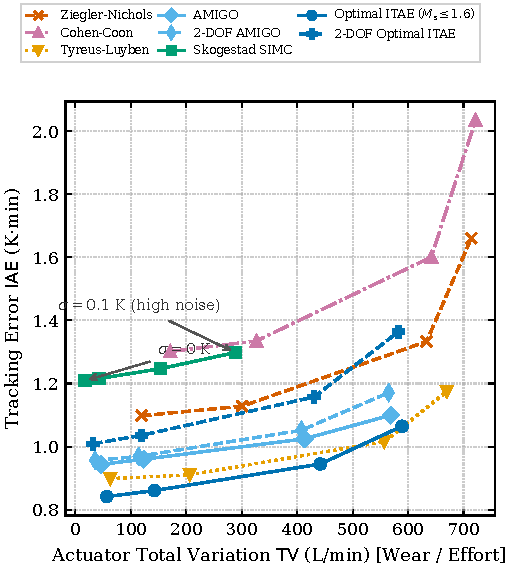
\includegraphics[width=0.92\columnwidth]{figures/fig_noise_sensitivity.pdf}
    \caption{Mean true-temperature IAE versus mean valve travel as the sensor noise grows from $\sigma = 0$ to $0.1$~K, with the measurement filter $\tau_m = 0.05$~min ($30$ runs per point).}
    \label{fig:noise_sensitivity}
\end{figure}

\begin{table*}[t]
\centering
\footnotesize
\caption{Sensitivity of tracking error (IAE) and actuator effort (TV) to measurement noise levels across $30$ Monte Carlo runs; $\tau_m$ is the time constant of the first-order measurement filter ($0$ = unfiltered).}
\label{tab:noise_sensitivity}
\resizebox{\ifdim\width>\textwidth\textwidth\else\width\fi}{!}{%
\begin{tabular}{lcccc}
\toprule
Method & $\tau_m$ (min) & Noise $\sigma$ (K) & IAE (mean $\pm$ 95\% CI) & TV (L/min) \\
\midrule
Ziegler-Nichols & 0.00 & 0.0 & 0.94 $\pm$ 0.00 & 81.9 $\pm$ 0.0 \\
Ziegler-Nichols & 0.00 & 0.01 & 1.00 $\pm$ 0.01 & 585.3 $\pm$ 4.3 \\
Ziegler-Nichols & 0.00 & 0.05 & 1.43 $\pm$ 0.03 & 748.9 $\pm$ 2.1 \\
Ziegler-Nichols & 0.00 & 0.1 & 2.03 $\pm$ 0.07 & 773.7 $\pm$ 1.7 \\
Ziegler-Nichols & 0.05 & 0.0 & 1.10 $\pm$ 0.00 & 119.5 $\pm$ 0.0 \\
Ziegler-Nichols & 0.05 & 0.01 & 1.13 $\pm$ 0.00 & 300.6 $\pm$ 2.1 \\
Ziegler-Nichols & 0.05 & 0.05 & 1.33 $\pm$ 0.03 & 633.5 $\pm$ 3.7 \\
Ziegler-Nichols & 0.05 & 0.1 & 1.66 $\pm$ 0.04 & 714.0 $\pm$ 3.4 \\
Cohen-Coon & 0.00 & 0.0 & 1.02 $\pm$ 0.00 & 104.0 $\pm$ 0.0 \\
Cohen-Coon & 0.00 & 0.01 & 1.08 $\pm$ 0.01 & 583.4 $\pm$ 4.7 \\
Cohen-Coon & 0.00 & 0.05 & 1.54 $\pm$ 0.04 & 749.3 $\pm$ 1.7 \\
Cohen-Coon & 0.00 & 0.1 & 2.12 $\pm$ 0.06 & 773.1 $\pm$ 1.7 \\
Cohen-Coon & 0.05 & 0.0 & 1.30 $\pm$ 0.00 & 171.0 $\pm$ 0.0 \\
Cohen-Coon & 0.05 & 0.01 & 1.34 $\pm$ 0.00 & 326.3 $\pm$ 2.0 \\
Cohen-Coon & 0.05 & 0.05 & 1.60 $\pm$ 0.03 & 641.8 $\pm$ 4.0 \\
Cohen-Coon & 0.05 & 0.1 & 2.04 $\pm$ 0.06 & 721.8 $\pm$ 2.8 \\
Tyreus-Luyben & 0.00 & 0.0 & 0.92 $\pm$ 0.00 & 48.8 $\pm$ 0.0 \\
Tyreus-Luyben & 0.00 & 0.01 & 0.96 $\pm$ 0.00 & 511.3 $\pm$ 4.5 \\
Tyreus-Luyben & 0.00 & 0.05 & 1.21 $\pm$ 0.02 & 722.5 $\pm$ 2.8 \\
Tyreus-Luyben & 0.00 & 0.1 & 1.51 $\pm$ 0.03 & 759.4 $\pm$ 2.8 \\
Tyreus-Luyben & 0.05 & 0.0 & 0.90 $\pm$ 0.00 & 62.9 $\pm$ 0.0 \\
Tyreus-Luyben & 0.05 & 0.01 & 0.91 $\pm$ 0.00 & 206.3 $\pm$ 1.6 \\
Tyreus-Luyben & 0.05 & 0.05 & 1.02 $\pm$ 0.01 & 557.2 $\pm$ 4.4 \\
Tyreus-Luyben & 0.05 & 0.1 & 1.17 $\pm$ 0.02 & 669.7 $\pm$ 3.1 \\
AMIGO & 0.00 & 0.0 & 0.93 $\pm$ 0.00 & 40.4 $\pm$ 0.0 \\
AMIGO & 0.00 & 0.01 & 0.94 $\pm$ 0.00 & 372.3 $\pm$ 4.0 \\
AMIGO & 0.00 & 0.05 & 1.05 $\pm$ 0.01 & 666.5 $\pm$ 3.5 \\
AMIGO & 0.00 & 0.1 & 1.24 $\pm$ 0.02 & 727.0 $\pm$ 2.9 \\
AMIGO & 0.05 & 0.0 & 0.94 $\pm$ 0.00 & 45.9 $\pm$ 0.0 \\
AMIGO & 0.05 & 0.01 & 0.96 $\pm$ 0.00 & 123.3 $\pm$ 0.9 \\
AMIGO & 0.05 & 0.05 & 1.02 $\pm$ 0.01 & 413.4 $\pm$ 3.4 \\
AMIGO & 0.05 & 0.1 & 1.10 $\pm$ 0.01 & 568.9 $\pm$ 4.1 \\
2-DOF AMIGO & 0.00 & 0.0 & 0.96 $\pm$ 0.00 & 29.3 $\pm$ 0.0 \\
2-DOF AMIGO & 0.00 & 0.01 & 1.00 $\pm$ 0.01 & 366.7 $\pm$ 4.0 \\
2-DOF AMIGO & 0.00 & 0.05 & 1.26 $\pm$ 0.02 & 664.4 $\pm$ 3.7 \\
2-DOF AMIGO & 0.00 & 0.1 & 1.53 $\pm$ 0.03 & 725.8 $\pm$ 2.8 \\
2-DOF AMIGO & 0.05 & 0.0 & 0.96 $\pm$ 0.00 & 35.5 $\pm$ 0.0 \\
2-DOF AMIGO & 0.05 & 0.01 & 0.97 $\pm$ 0.00 & 113.9 $\pm$ 1.0 \\
2-DOF AMIGO & 0.05 & 0.05 & 1.05 $\pm$ 0.01 & 407.7 $\pm$ 3.5 \\
2-DOF AMIGO & 0.05 & 0.1 & 1.17 $\pm$ 0.01 & 565.1 $\pm$ 4.1 \\
Skogestad SIMC & 0.00 & 0.0 & 1.29 $\pm$ 0.00 & 15.7 $\pm$ 0.0 \\
Skogestad SIMC & 0.00 & 0.01 & 1.29 $\pm$ 0.00 & 133.2 $\pm$ 1.7 \\
Skogestad SIMC & 0.00 & 0.05 & 1.44 $\pm$ 0.02 & 474.1 $\pm$ 4.6 \\
Skogestad SIMC & 0.00 & 0.1 & 1.71 $\pm$ 0.03 & 603.0 $\pm$ 4.3 \\
Skogestad SIMC & 0.05 & 0.0 & 1.21 $\pm$ 0.00 & 17.2 $\pm$ 0.0 \\
Skogestad SIMC & 0.05 & 0.01 & 1.22 $\pm$ 0.00 & 42.7 $\pm$ 0.3 \\
Skogestad SIMC & 0.05 & 0.05 & 1.25 $\pm$ 0.00 & 153.0 $\pm$ 1.6 \\
Skogestad SIMC & 0.05 & 0.1 & 1.30 $\pm$ 0.01 & 288.3 $\pm$ 2.9 \\
Optimal ITAE ($M_s \leq 1.6$) & 0.00 & 0.0 & 0.83 $\pm$ 0.00 & 48.6 $\pm$ 0.0 \\
Optimal ITAE ($M_s \leq 1.6$) & 0.00 & 0.01 & 0.85 $\pm$ 0.00 & 400.6 $\pm$ 4.2 \\
Optimal ITAE ($M_s \leq 1.6$) & 0.00 & 0.05 & 1.03 $\pm$ 0.01 & 677.9 $\pm$ 3.7 \\
Optimal ITAE ($M_s \leq 1.6$) & 0.00 & 0.1 & 1.27 $\pm$ 0.02 & 734.1 $\pm$ 2.6 \\
Optimal ITAE ($M_s \leq 1.6$) & 0.05 & 0.0 & 0.84 $\pm$ 0.00 & 56.6 $\pm$ 0.0 \\
Optimal ITAE ($M_s \leq 1.6$) & 0.05 & 0.01 & 0.86 $\pm$ 0.00 & 142.3 $\pm$ 1.0 \\
Optimal ITAE ($M_s \leq 1.6$) & 0.05 & 0.05 & 0.94 $\pm$ 0.01 & 441.8 $\pm$ 3.8 \\
Optimal ITAE ($M_s \leq 1.6$) & 0.05 & 0.1 & 1.06 $\pm$ 0.01 & 589.2 $\pm$ 4.2 \\
2-DOF Optimal ITAE & 0.00 & 0.0 & 1.08 $\pm$ 0.00 & 25.0 $\pm$ 0.0 \\
2-DOF Optimal ITAE & 0.00 & 0.01 & 1.13 $\pm$ 0.01 & 389.7 $\pm$ 4.2 \\
2-DOF Optimal ITAE & 0.00 & 0.05 & 1.50 $\pm$ 0.02 & 675.0 $\pm$ 3.4 \\
2-DOF Optimal ITAE & 0.00 & 0.1 & 1.80 $\pm$ 0.03 & 732.5 $\pm$ 2.6 \\
2-DOF Optimal ITAE & 0.05 & 0.0 & 1.01 $\pm$ 0.00 & 31.3 $\pm$ 0.0 \\
2-DOF Optimal ITAE & 0.05 & 0.01 & 1.04 $\pm$ 0.01 & 119.4 $\pm$ 1.0 \\
2-DOF Optimal ITAE & 0.05 & 0.05 & 1.16 $\pm$ 0.02 & 430.3 $\pm$ 3.6 \\
2-DOF Optimal ITAE & 0.05 & 0.1 & 1.36 $\pm$ 0.02 & 582.8 $\pm$ 4.0 \\
\bottomrule
\end{tabular}%
}
\end{table*}


\begin{table*}[t]
\centering
\footnotesize
\caption{Effect of the measurement filter ($\tau_m = 0.05$~min against none) on the $30$ paired noise realizations: mean paired difference and Wilcoxon signed-rank $p$-values adjusted by Benjamini--Hochberg over all tests in the table.}
\label{tab:noise_filter_paired}
\resizebox{\ifdim\width>\textwidth\textwidth\else\width\fi}{!}{%
\begin{tabular}{lccccc}
\toprule
Method & Noise $\sigma$ (K) & \(\Delta\)TV (L/min) & \(p_{\mathrm{adj}}\) (TV) & \(\Delta\)IAE (K$\cdot$min) & \(p_{\mathrm{adj}}\) (IAE) \\
\midrule
Ziegler-Nichols & 0.01 & -284.8 & $<10^{-3}$ & +0.127 & $<10^{-3}$ \\
Ziegler-Nichols & 0.05 & -115.4 & $<10^{-3}$ & -0.100 & $<10^{-3}$ \\
Ziegler-Nichols & 0.10 & -59.7 & $<10^{-3}$ & -0.370 & $<10^{-3}$ \\
Cohen-Coon & 0.01 & -257.1 & $<10^{-3}$ & +0.255 & $<10^{-3}$ \\
Cohen-Coon & 0.05 & -107.5 & $<10^{-3}$ & +0.059 & 0.020 \\
Cohen-Coon & 0.10 & -51.3 & $<10^{-3}$ & -0.085 & 0.040 \\
Tyreus-Luyben & 0.01 & -305.0 & $<10^{-3}$ & -0.046 & $<10^{-3}$ \\
Tyreus-Luyben & 0.05 & -165.3 & $<10^{-3}$ & -0.192 & $<10^{-3}$ \\
Tyreus-Luyben & 0.10 & -89.7 & $<10^{-3}$ & -0.334 & $<10^{-3}$ \\
AMIGO & 0.01 & -249.0 & $<10^{-3}$ & +0.016 & $<10^{-3}$ \\
AMIGO & 0.05 & -253.2 & $<10^{-3}$ & -0.023 & $<10^{-3}$ \\
AMIGO & 0.10 & -158.0 & $<10^{-3}$ & -0.136 & $<10^{-3}$ \\
2-DOF AMIGO & 0.01 & -252.8 & $<10^{-3}$ & -0.033 & $<10^{-3}$ \\
2-DOF AMIGO & 0.05 & -256.8 & $<10^{-3}$ & -0.213 & $<10^{-3}$ \\
2-DOF AMIGO & 0.10 & -160.6 & $<10^{-3}$ & -0.357 & $<10^{-3}$ \\
Skogestad SIMC & 0.01 & -90.5 & $<10^{-3}$ & -0.078 & $<10^{-3}$ \\
Skogestad SIMC & 0.05 & -321.1 & $<10^{-3}$ & -0.194 & $<10^{-3}$ \\
Skogestad SIMC & 0.10 & -314.7 & $<10^{-3}$ & -0.410 & $<10^{-3}$ \\
Optimal ITAE ($M_s \leq 1.6$) & 0.01 & -258.3 & $<10^{-3}$ & +0.012 & $<10^{-3}$ \\
Optimal ITAE ($M_s \leq 1.6$) & 0.05 & -236.1 & $<10^{-3}$ & -0.080 & $<10^{-3}$ \\
Optimal ITAE ($M_s \leq 1.6$) & 0.10 & -144.8 & $<10^{-3}$ & -0.210 & $<10^{-3}$ \\
2-DOF Optimal ITAE & 0.01 & -270.3 & $<10^{-3}$ & -0.090 & $<10^{-3}$ \\
2-DOF Optimal ITAE & 0.05 & -244.7 & $<10^{-3}$ & -0.341 & $<10^{-3}$ \\
2-DOF Optimal ITAE & 0.10 & -149.7 & $<10^{-3}$ & -0.433 & $<10^{-3}$ \\
\bottomrule
\end{tabular}%
}
\end{table*}


Since the IAE is evaluated on the true temperature, the table measures how much sensor noise each loop converts into real thermal deviation. Without the filter, valve travel is bounded by $|u_0 - \bar q_j| + S_{\max}t_f \approx 800$~L/min and approaches this ceiling quickly: at $\sigma = 0.01$~K the travel is already $585.3$ (ZN), $583.4$ (CC) and $511.3$~L/min (TL), and at $0.1$~K every tuning except SIMC ($603.0$~L/min) lies between $725.8$ and $773.7$~L/min, which hides differences in valve wear. The ordering follows the high-frequency gain of Table~\ref{tab:exact_robustness}: ZN and CC, with $K_{\mathrm{hf}}$ of $490$ and $559$~L/min/K, are the noisiest, SIMC ($77$~L/min/K) the quietest.

The filter spreads the tunings out. At $\sigma = 0.01$~K the travel falls by a factor of $1.8$ to $3.3$ (ZN $585.3 \rightarrow 300.6$, TL $511.3 \rightarrow 206.3$, AMIGO $372.3 \rightarrow 123.3$, Optimal ITAE $400.6 \rightarrow 142.3$, SIMC $133.2 \rightarrow 42.7$~L/min), and the ratio between the noisiest and the quietest tuning grows from $4.4$ to $7.6$. At $\sigma = 0.05$~K the range is $153.0$ (SIMC) to $641.8$~L/min (CC). The filter is not sufficient for the empirical rules at $\sigma = 0.1$~K, where ZN and CC still reach $714.0$ and $721.8$~L/min, within $11\%$ of the ceiling, against $288.3$ for SIMC; a lower $N$ or a larger $\tau_m$ is needed there. All $24$ paired travel differences are significant after Benjamini--Hochberg adjustment ($p_{\mathrm{adj}} < 10^{-3}$), but with effects of $51$ to $321$~L/min against intervals of a few L/min the $p$-values carry no information; the relevant quantity is the size of the effect, a reduction of $7\%$ (CC, $\sigma = 0.1$~K) to $69\%$ (2-DOF AMIGO and 2-DOF Optimal ITAE, $\sigma = 0.01$~K) of the unfiltered travel (Table~\ref{tab:noise_filter_paired}). The effect on the tracking error depends on the noise level: at $\sigma = 0.01$~K the filter \emph{increases} the IAE of ZN ($+0.127$~K$\cdot$min) and CC ($+0.255$), consistent with phase lag outweighing the small noise reduction, and marginally that of AMIGO ($+0.016$) and Optimal ITAE ($+0.012$); at $\sigma \ge 0.05$~K it lowers the IAE of every tuning except CC at $0.05$~K ($+0.059$). The cost is the phase lag of the filter in the noise-free loop (IAE $0.94 \rightarrow 1.10$ for ZN and $1.02 \rightarrow 1.30$~K$\cdot$min for CC, but $0.83 \rightarrow 0.84$ for Optimal ITAE and $1.29 \rightarrow 1.21$ for SIMC). With the filter at $\sigma = 0.1$~K the true-temperature error ranks Optimal ITAE ($1.06 \pm 0.01$~K$\cdot$min), AMIGO ($1.10 \pm 0.01$), TL ($1.17 \pm 0.02$) and SIMC ($1.30 \pm 0.01$) ahead of ZN ($1.66 \pm 0.04$) and CC ($2.04 \pm 0.06$), with non-overlapping $95\%$ intervals.

\paragraph{The derivative-filter coefficient as a design variable.} The high-frequency gain $K_{\mathrm{hf}} = |K_p|(1+N)$ depends on $N$ as much as on the tuning rule, and the benchmark uses $N = 10$ for every rule. Table~\ref{tab:n_design} lowers $N$ for ZN and CC: $N = 3$ cuts $K_{\mathrm{hf}}$ by $64\%$ ($490 \rightarrow 178$ and $559 \rightarrow 203$~L/min/K) without changing the noise-free IAE ($0.940 \rightarrow 0.942$ and $1.017 \rightarrow 1.010$~K$\cdot$min), and at $\sigma = 0.01$~K it reduces the travel from $585$ to $529$~L/min (ZN) and from $583$ to $543$ (CC), i.e.\ $10\%$ and $7\%$. At $\sigma = 0.05$~K the travel stays between $731$ and $749$~L/min, near the $800$~L/min ceiling, for every $N$. A smaller $N$ is thus a free reduction of noise gain for these rules, but it is a weaker remedy than the measurement filter ($-49\%$ and $-44\%$ at $\sigma = 0.01$~K), and it does not remove the discrimination problem of TV at large noise.

\begin{table*}[t]
\centering
\footnotesize
\caption{Derivative-filter coefficient $N$ ($\tau_f = T_d/N$) as a design variable for the empirical rules, $-2$~K step, unfiltered measurement; $K_{\mathrm{hf}} = |K_p|(1+N)$ equals $\|CS\|_\infty$ to within $0.3$~L/min/K in every row. Noise columns: mean $\pm$ $95\%$ half-width over 30 realizations; TV in L/min, IAE in K$\cdot$min.}
\label{tab:n_design}
\resizebox{\ifdim\width>\textwidth\textwidth\else\width\fi}{!}{%
\begin{tabular}{lcccccccc}
\toprule
Method & \(N\) & \(K_{\mathrm{hf}}\) (L/min/K) & IAE (noise-free) & \(M_p\) (\%) & IAE ($\sigma=0.01$) & TV ($\sigma=0.01$) & IAE ($\sigma=0.05$) & TV ($\sigma=0.05$) \\
\midrule
Ziegler-Nichols & 3 & 178 & 0.942 & 23.3 & 0.99 $\pm$ 0.01 & 529 $\pm$ 4 & 1.29 $\pm$ 0.03 & 731 $\pm$ 3 \\
Ziegler-Nichols & 5 & 267 & 0.941 & 22.9 & 0.99 $\pm$ 0.01 & 558 $\pm$ 4 & 1.34 $\pm$ 0.03 & 742 $\pm$ 2 \\
Ziegler-Nichols & 10 & 490 & 0.940 & 22.6 & 1.00 $\pm$ 0.01 & 585 $\pm$ 4 & 1.43 $\pm$ 0.03 & 749 $\pm$ 2 \\
Cohen-Coon & 3 & 203 & 1.010 & 31.4 & 1.07 $\pm$ 0.01 & 543 $\pm$ 5 & 1.44 $\pm$ 0.03 & 736 $\pm$ 2 \\
Cohen-Coon & 5 & 305 & 1.011 & 31.1 & 1.07 $\pm$ 0.01 & 564 $\pm$ 5 & 1.49 $\pm$ 0.03 & 743 $\pm$ 2 \\
Cohen-Coon & 10 & 559 & 1.017 & 31.0 & 1.08 $\pm$ 0.01 & 583 $\pm$ 5 & 1.54 $\pm$ 0.04 & 749 $\pm$ 2 \\
\bottomrule
\end{tabular}%
}
\end{table*}


\section{Load disturbances: replicated runs}\label{supp:load}
\subsection{Unmeasured load disturbances}
\label{supp:loadfull}
A feed temperature step $\Delta T_f = +2$~K at $t = 2$~min and a feed concentration step $\Delta C_{Af} = +0.1$~mol/L ($+10\%$) at $t = 8$~min were applied at constant setpoint. Table~\ref{tab:load_disturbance} is the deterministic response (no noise, no measurement filter) and ranks the loops without sampling uncertainty; Table~\ref{tab:load_replicated} repeats the run with $30$ independent noise realizations ($\sigma = 0.05$~K), without and with the measurement filter ($\tau_m = 0.05$~min), and reports mean $\pm$ the half-width of the $95\%$ $t$-interval (Fig.~\ref{fig:disturbance_rejection} shows the deterministic response).

\begin{figure*}[t]
    \centering
    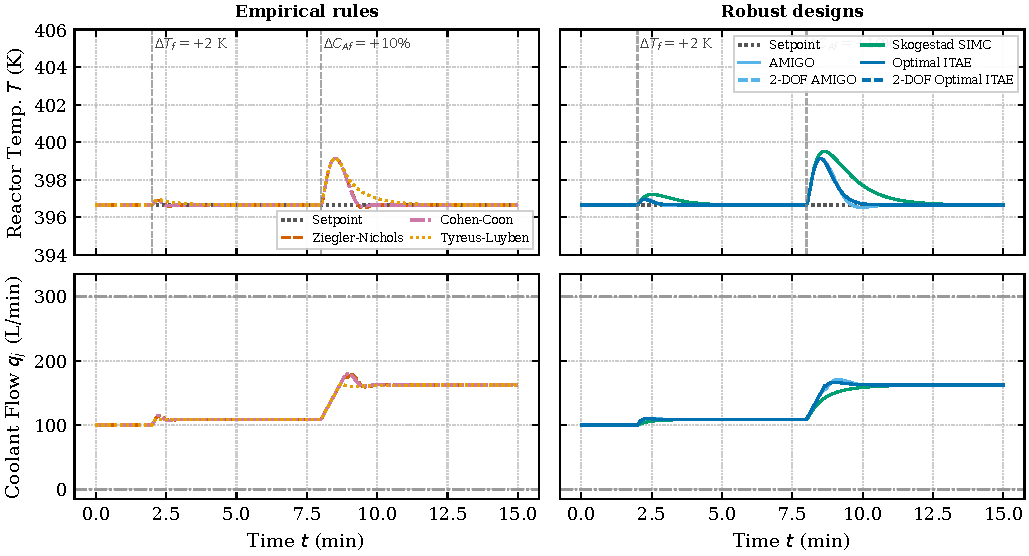
\includegraphics[width=0.92\textwidth]{figures/fig2_disturbance_rejection.pdf}
    \caption{Deterministic rejection of a $+2$~K feed temperature step at $t = 2$~min and a $+10\%$ feed concentration step at $t = 8$~min: empirical rules (left) and robust designs (right).}
    \label{fig:disturbance_rejection}
\end{figure*}

\begin{table*}[t]
\centering
\footnotesize
\caption{Regulatory performance under combined feed temperature ($+2$~K) and concentration ($+10\%$) load disturbances. $T(t_f) - T_{sp}$ is the true temperature error at $t_f = 15$~min.}
\label{tab:load_disturbance}
\resizebox{\ifdim\width>\textwidth\textwidth\else\width\fi}{!}{%
\begin{tabular}{lcccccc}
\toprule
Method & IAE & ITAE (K$\cdot$min$^2$) & TV (L/min) & Peak Dev (K) & Max Valve (L/min) & \(T(t_f) - T_{sp}\) (K) \\
\midrule
Ziegler-Nichols & 2.38 & 19.48 & 1116.7 & 2.51 & 177.9 & -0.07 \\
Cohen-Coon & 2.39 & 19.43 & 1117.0 & 2.49 & 178.2 & -0.06 \\
Tyreus-Luyben & 4.16 & 36.46 & 1077.6 & 2.54 & 166.2 & +0.02 \\
AMIGO & 3.01 & 24.64 & 991.1 & 2.53 & 167.5 & +0.01 \\
2-DOF AMIGO & 3.01 & 24.64 & 991.1 & 2.53 & 167.5 & +0.01 \\
Skogestad SIMC & 7.05 & 62.23 & 692.8 & 3.07 & 163.7 & +0.04 \\
Optimal ITAE ($M_s \leq 1.6$) & 3.23 & 27.04 & 1011.1 & 2.51 & 165.4 & +0.00 \\
2-DOF Optimal ITAE & 3.23 & 27.04 & 1011.1 & 2.51 & 165.4 & +0.00 \\
\bottomrule
\end{tabular}%
}
\end{table*}


\begin{table*}[t]
\centering
\footnotesize
\caption{Load profile of Section~\ref{subsec:load_results} with 30 independent noise realizations ($\sigma = 0.05$~K), without ($\tau_m = 0$) and with ($\tau_m = 0.05$~min) measurement filter: mean $\pm$ half-width of the $95\%$ $t$-interval. Errors are measured on the true temperature; the TV ceiling is $S_{\max}t_f = 1200$~L/min.}
\label{tab:load_replicated}
\resizebox{\ifdim\width>\textwidth\textwidth\else\width\fi}{!}{%
\begin{tabular}{lccccc}
\toprule
Method & \(\tau_m\) (min) & IAE & Peak dev. (K) & TV (L/min) & TV/ceiling (\%) \\
\midrule
Ziegler-Nichols & 0.00 & 2.59 $\pm$ 0.07 & 2.54 $\pm$ 0.06 & 1114 $\pm$ 4 & 93 \\
Ziegler-Nichols & 0.05 & 2.41 $\pm$ 0.05 & 2.57 $\pm$ 0.04 & 933 $\pm$ 6 & 78 \\
Cohen-Coon & 0.00 & 2.59 $\pm$ 0.08 & 2.55 $\pm$ 0.07 & 1112 $\pm$ 4 & 93 \\
Cohen-Coon & 0.05 & 2.41 $\pm$ 0.05 & 2.58 $\pm$ 0.04 & 924 $\pm$ 6 & 77 \\
Tyreus-Luyben & 0.00 & 4.31 $\pm$ 0.06 & 2.59 $\pm$ 0.05 & 1077 $\pm$ 4 & 90 \\
Tyreus-Luyben & 0.05 & 3.50 $\pm$ 0.04 & 2.58 $\pm$ 0.03 & 828 $\pm$ 7 & 69 \\
AMIGO & 0.00 & 3.13 $\pm$ 0.04 & 2.59 $\pm$ 0.03 & 997 $\pm$ 6 & 83 \\
AMIGO & 0.05 & 2.69 $\pm$ 0.02 & 2.60 $\pm$ 0.02 & 621 $\pm$ 7 & 52 \\
2-DOF AMIGO & 0.00 & 3.13 $\pm$ 0.04 & 2.59 $\pm$ 0.03 & 997 $\pm$ 6 & 83 \\
2-DOF AMIGO & 0.05 & 2.69 $\pm$ 0.02 & 2.60 $\pm$ 0.02 & 621 $\pm$ 7 & 52 \\
Skogestad SIMC & 0.00 & 7.25 $\pm$ 0.07 & 3.05 $\pm$ 0.01 & 704 $\pm$ 6 & 59 \\
Skogestad SIMC & 0.05 & 5.83 $\pm$ 0.02 & 3.03 $\pm$ 0.01 & 243 $\pm$ 3 & 20 \\
Optimal ITAE ($M_s^{\mathrm{FOPTD}} \leq 1.6$) & 0.00 & 3.33 $\pm$ 0.04 & 2.58 $\pm$ 0.03 & 1011 $\pm$ 6 & 84 \\
Optimal ITAE ($M_s^{\mathrm{FOPTD}} \leq 1.6$) & 0.05 & 2.75 $\pm$ 0.03 & 2.60 $\pm$ 0.02 & 655 $\pm$ 7 & 55 \\
2-DOF Optimal ITAE & 0.00 & 3.33 $\pm$ 0.04 & 2.58 $\pm$ 0.03 & 1011 $\pm$ 6 & 84 \\
2-DOF Optimal ITAE & 0.05 & 2.75 $\pm$ 0.03 & 2.60 $\pm$ 0.02 & 655 $\pm$ 7 & 55 \\
\bottomrule
\end{tabular}%
}
\end{table*}


The magnitudes are chosen so that the heat-removal demand leaves the valve room to act: a first campaign with $+5$~K and $+20\%$ drove every loop to within $15$~L/min of the upper stop, where saturation, not the controller, decided the response; here the largest valve opening is $162.4$--$180.0$~L/min, far from the $300$~L/min stop. All loops return to the setpoint by integral action ($|T(t_f) - T_{sp}| \le 0.01$~K). The peak deviation is $2.49$~K for ZN, CC, TL, AMIGO and Optimal ITAE and $2.86$~K for SIMC: its equality across five different tunings indicates that it is set by the plant delay and the slew rate rather than by the tuning, so it is not a discriminating metric. The deterministic IAE ranks CC ($1.98$~K$\cdot$min), ZN ($2.04$), AMIGO ($2.42$) and Optimal ITAE ($2.43$) ahead of TL ($3.02$) and SIMC ($5.70$), and the $30$ replications confirm the order with non-overlapping $95\%$ intervals in every comparison except between ZN and CC (unfiltered: $2.59 \pm 0.07$ and $2.59 \pm 0.08$; filtered: $2.41 \pm 0.05$ for both). The ranking differs from the servo ranking: Optimal ITAE, the fastest servo loop, is fourth in regulation, and the empirical rules lead. TV is reported but not used to rank: in the noise-free response it is $5$--$11\%$ of the ceiling and does discriminate ($62.4$ for SIMC to $129.3$~L/min for ZN), but with measurement noise the unfiltered empirical rules sit at $93\%$ of the $1200$~L/min ceiling ($1114 \pm 4$ and $1112 \pm 4$~L/min) and the filtered ones at $77$--$78\%$, where the ceiling, not the loop, bounds the difference. The 2-DOF variants reproduce their 1-DOF metrics exactly (e.g.\ AMIGO and 2-DOF AMIGO: $2.42$~K$\cdot$min), which confirms that setpoint weighting does not alter the disturbance response. This regulation ranking is specific to the regime of this study, in which the rate limit dominates the peak deviation; with a faster valve or a larger disturbance the peak, and the ranking, would be set by other limits.

\section{Global sensitivity under simultaneous uncertainty}\label{supp:sobol}
\subsection{Global sensitivity under simultaneous uncertainty}
\label{subsec:sobol_results}
Sobol' indices \cite{sobol2001global, saltelli2010variance} decompose the variance of a closed-loop metric $Y \in \{\mathrm{IAE}, \mathrm{TV}\}$ over uncertain factors $\boldsymbol{\xi}$:
\begin{equation}
    S_i = \frac{\mathbb{V}_{\xi_i}\!\left[\mathbb{E}(Y \mid \xi_i)\right]}{\mathbb{V}(Y)}, \qquad S_{Ti} = \frac{\mathbb{E}_{\boldsymbol{\xi}_{\sim i}}\!\left[\mathbb{V}(Y \mid \boldsymbol{\xi}_{\sim i})\right]}{\mathbb{V}(Y)},
    \label{eq:sobol}
\end{equation}
where $S_i$ is the share of variance explained by $\xi_i$ alone and $S_{Ti} \ge S_i$ adds its interactions. The factors were sampled uniformly on $E_a/R \in [0.97, 1.03]$, $UA \in [0.65, 1.05]$ (both relative to nominal), $C_{Af} \in [0.85, 1.15]$~mol/L and a pure sensor dead time $\theta_{\text{sensor}} \in [0, 0.1]$~min. Every run starts from the \emph{nominal} equilibrium and applies a $-2$~K step at $t = 0.5$~min on the perturbed plant (the half minute fills the sensor delay line), so the response contains the transient caused by the parametric deviation as well as the step. The loop is the benchmark loop: the valve limits of Section~\ref{subsec:actuator_limits}, the directional amplitude-plus-rate clamping of Eq.~\eqref{eq:clamping_antiwindup}, $\Delta t = 0.02$~min and $10$~min after the step, as in the nominal protocol. Indices were estimated with Saltelli sampling and the SALib estimators \cite{herman2017salib} ($N = 512$, $3072$ runs per tuning) for seven tunings (Fig.~\ref{fig:sobol}, Table~\ref{tab:sobol_sensitivity}); the intervals are the half-widths of the $95\%$ bootstrap intervals of SALib (100 resamples), and every table satisfies $S_{Ti} \ge S_i - 0.01$.

\paragraph{Ranges.} The box is asymmetric by design: fouling can only reduce $UA$ (to $65\%$) and the $+5\%$ allows for calibration error, whereas $E_a/R$ is known more tightly than the feed concentration. Because a Sobol' index is relative to the chosen box, Table~\ref{tab:sobol_ranges} expresses each range as the coolant flow needed to hold the new setpoint when one factor sits at a bound and the others are nominal. The $UA$ and $C_{Af}$ ranges move the heat-removal demand by about $170$ and $148$~L/min, the $E_a/R$ range by about $33$~L/min: the ranking of the factors below reflects these ranges, and a narrower $UA$ or $C_{Af}$ box would be expected to shift variance towards $E_a/R$.

\begin{figure*}[t]
    \centering
    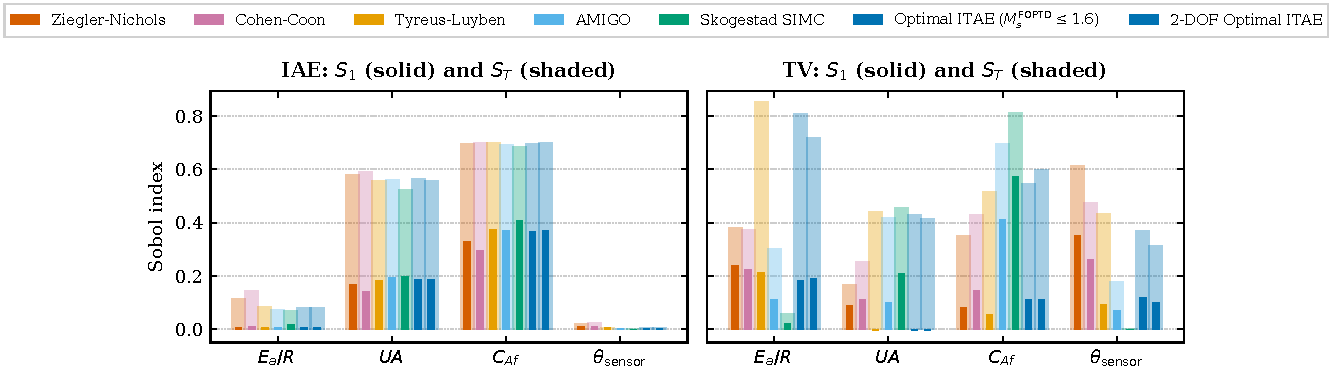
\includegraphics[width=0.92\textwidth]{figures/fig_sobol_indices.pdf}
    \caption{First-order ($S_1$, solid) and total-order ($S_T$, shaded) Sobol indices of IAE (left) and TV (right) for seven PID tunings.}
    \label{fig:sobol}
\end{figure*}

\begin{table*}[t]
\centering
\footnotesize
\caption{Global Sobol indices (Saltelli sampling, $N=512$, $3072$ closed-loop runs per controller) of IAE and TV for a $-2$~K setpoint step at $t = 0.5$~min under simultaneous uncertainty $E_a/R \in [0.97, 1.03]$, $UA \in [0.65, 1.05]\,UA_{\mathrm{nom}}$, $C_{Af} \in [0.85, 1.15]$~mol/L and sensor dead time $\theta_{\mathrm{sensor}} \in [0, 0.1]$~min. Every run starts from the nominal equilibrium, uses the directional amplitude-plus-rate clamping of Eq.~\eqref{eq:clamping_antiwindup} with $\Delta t = 0.02$~min and lasts $10$~min after the step. Entries are index $\pm$ half-width of the $95\%$ bootstrap interval (SALib, 100 resamples).}
\label{tab:sobol_sensitivity}
\resizebox{\ifdim\width>\textwidth\textwidth\else\width\fi}{!}{%
\begin{tabular}{lccccc}
\toprule
Controller & Parameter & $S_1$ (IAE) & $S_T$ (IAE) & $S_1$ (TV) & $S_T$ (TV) \\
\midrule
Ziegler-Nichols & $E_a/R$ & 0.006 $\pm$ 0.025 & 0.112 $\pm$ 0.033 & 0.237 $\pm$ 0.077 & 0.379 $\pm$ 0.073 \\
Ziegler-Nichols & $UA$ & 0.169 $\pm$ 0.103 & 0.580 $\pm$ 0.131 & 0.087 $\pm$ 0.052 & 0.166 $\pm$ 0.033 \\
Ziegler-Nichols & $C_{Af}$ & 0.329 $\pm$ 0.122 & 0.695 $\pm$ 0.172 & 0.083 $\pm$ 0.079 & 0.349 $\pm$ 0.066 \\
Ziegler-Nichols & $\theta_{\mathrm{sensor}}$ & 0.011 $\pm$ 0.012 & 0.018 $\pm$ 0.008 & 0.351 $\pm$ 0.089 & 0.612 $\pm$ 0.083 \\
Cohen-Coon & $E_a/R$ & 0.009 $\pm$ 0.031 & 0.142 $\pm$ 0.040 & 0.223 $\pm$ 0.075 & 0.371 $\pm$ 0.068 \\
Cohen-Coon & $UA$ & 0.142 $\pm$ 0.101 & 0.588 $\pm$ 0.130 & 0.112 $\pm$ 0.061 & 0.251 $\pm$ 0.047 \\
Cohen-Coon & $C_{Af}$ & 0.295 $\pm$ 0.120 & 0.700 $\pm$ 0.168 & 0.146 $\pm$ 0.082 & 0.430 $\pm$ 0.067 \\
Cohen-Coon & $\theta_{\mathrm{sensor}}$ & 0.011 $\pm$ 0.016 & 0.025 $\pm$ 0.009 & 0.262 $\pm$ 0.083 & 0.473 $\pm$ 0.069 \\
Tyreus-Luyben & $E_a/R$ & 0.008 $\pm$ 0.023 & 0.084 $\pm$ 0.025 & 0.213 $\pm$ 0.105 & 0.851 $\pm$ 0.266 \\
Tyreus-Luyben & $UA$ & 0.183 $\pm$ 0.099 & 0.556 $\pm$ 0.126 & -0.006 $\pm$ 0.066 & 0.439 $\pm$ 0.202 \\
Tyreus-Luyben & $C_{Af}$ & 0.373 $\pm$ 0.122 & 0.699 $\pm$ 0.172 & 0.054 $\pm$ 0.122 & 0.515 $\pm$ 0.164 \\
Tyreus-Luyben & $\theta_{\mathrm{sensor}}$ & 0.005 $\pm$ 0.007 & 0.006 $\pm$ 0.003 & 0.093 $\pm$ 0.092 & 0.433 $\pm$ 0.218 \\
AMIGO & $E_a/R$ & 0.008 $\pm$ 0.023 & 0.072 $\pm$ 0.022 & 0.112 $\pm$ 0.075 & 0.301 $\pm$ 0.079 \\
AMIGO & $UA$ & 0.194 $\pm$ 0.102 & 0.559 $\pm$ 0.127 & 0.100 $\pm$ 0.105 & 0.416 $\pm$ 0.107 \\
AMIGO & $C_{Af}$ & 0.370 $\pm$ 0.123 & 0.689 $\pm$ 0.172 & 0.410 $\pm$ 0.158 & 0.696 $\pm$ 0.097 \\
AMIGO & $\theta_{\mathrm{sensor}}$ & 0.001 $\pm$ 0.003 & 0.000 $\pm$ 0.000 & 0.070 $\pm$ 0.095 & 0.179 $\pm$ 0.085 \\
Skogestad SIMC & $E_a/R$ & 0.017 $\pm$ 0.025 & 0.069 $\pm$ 0.020 & 0.020 $\pm$ 0.027 & 0.058 $\pm$ 0.012 \\
Skogestad SIMC & $UA$ & 0.200 $\pm$ 0.094 & 0.523 $\pm$ 0.115 & 0.208 $\pm$ 0.078 & 0.454 $\pm$ 0.073 \\
Skogestad SIMC & $C_{Af}$ & 0.407 $\pm$ 0.120 & 0.684 $\pm$ 0.163 & 0.575 $\pm$ 0.093 & 0.813 $\pm$ 0.121 \\
Skogestad SIMC & $\theta_{\mathrm{sensor}}$ & 0.000 $\pm$ 0.001 & 0.000 $\pm$ 0.000 & -0.001 $\pm$ 0.003 & 0.001 $\pm$ 0.000 \\
Optimal ITAE ($M_s^{\mathrm{FOPTD}} \leq 1.6$) & $E_a/R$ & 0.007 $\pm$ 0.024 & 0.078 $\pm$ 0.023 & 0.184 $\pm$ 0.088 & 0.807 $\pm$ 0.249 \\
Optimal ITAE ($M_s^{\mathrm{FOPTD}} \leq 1.6$) & $UA$ & 0.187 $\pm$ 0.100 & 0.562 $\pm$ 0.128 & -0.007 $\pm$ 0.066 & 0.428 $\pm$ 0.165 \\
Optimal ITAE ($M_s^{\mathrm{FOPTD}} \leq 1.6$) & $C_{Af}$ & 0.368 $\pm$ 0.122 & 0.696 $\pm$ 0.172 & 0.112 $\pm$ 0.166 & 0.545 $\pm$ 0.173 \\
Optimal ITAE ($M_s^{\mathrm{FOPTD}} \leq 1.6$) & $\theta_{\mathrm{sensor}}$ & 0.003 $\pm$ 0.005 & 0.003 $\pm$ 0.002 & 0.119 $\pm$ 0.118 & 0.369 $\pm$ 0.171 \\
2-DOF Optimal ITAE & $E_a/R$ & 0.007 $\pm$ 0.024 & 0.081 $\pm$ 0.024 & 0.192 $\pm$ 0.092 & 0.719 $\pm$ 0.222 \\
2-DOF Optimal ITAE & $UA$ & 0.185 $\pm$ 0.099 & 0.557 $\pm$ 0.126 & -0.004 $\pm$ 0.074 & 0.414 $\pm$ 0.167 \\
2-DOF Optimal ITAE & $C_{Af}$ & 0.371 $\pm$ 0.122 & 0.698 $\pm$ 0.171 & 0.113 $\pm$ 0.150 & 0.596 $\pm$ 0.174 \\
2-DOF Optimal ITAE & $\theta_{\mathrm{sensor}}$ & 0.004 $\pm$ 0.005 & 0.004 $\pm$ 0.003 & 0.102 $\pm$ 0.093 & 0.311 $\pm$ 0.137 \\
\bottomrule
\end{tabular}%
}
\end{table*}


\begin{table*}[t]
\centering
\footnotesize
\caption{Uncertainty box of the Sobol analysis expressed as heat-removal demand: coolant flow needed at the $-2$~K setpoint when one factor sits at a bound and the others are nominal (nominal: $110.9$~L/min; valve stop $300$~L/min). Ranges of $E_a/R$ and $UA$ are relative to nominal.}
\label{tab:sobol_ranges}
\resizebox{\ifdim\width>\textwidth\textwidth\else\width\fi}{!}{%
\begin{tabular}{lccc}
\toprule
Factor & Range & \(u_{\mathrm{req}}\), low (L/min) & \(u_{\mathrm{req}}\), high (L/min) \\
\midrule
$E_a/R$ & [0.97, 1.03] & 124.0 & 90.8 \\
$UA$ & [0.65, 1.05] & 275.1 & 105.3 \\
$C_{Af}$ & [0.85, 1.15] & 60.3 & 208.1 \\
$\theta_{\mathrm{sensor}}$ & [0, 0.1] & -- & -- \\
\bottomrule
\end{tabular}%
}
\end{table*}


\paragraph{Reading with the intervals.} The intervals are wide ($\pm 0.11$ to $\pm 0.17$ on the total-order index of IAE for the two leading factors, up to $\pm 0.27$ for TV), and they restrict what can be read from the point estimates. For every tuning the variance of IAE is explained mainly by feed concentration ($S_T = 0.684$--$0.700$) and heat-transfer capacity ($S_T = 0.523$--$0.588$), whereas the activation energy ($S_T = 0.069$--$0.142$) and the sensor dead time ($S_T \le 0.025$) contribute little; the two leading factors are resolved from the two minor ones, but not from each other, and the seven tunings are not distinguishable in the IAE decomposition. Valve activity does tell them apart. For SIMC the variance of TV follows the physical load ($C_{Af}$: $S_T = 0.813 \pm 0.121$) and is insensitive to the sensor delay ($S_T = 0.001$), while for ZN the TV is dominated by $\theta_{\text{sensor}}$ ($S_1 = 0.351 \pm 0.089$, $S_T = 0.612 \pm 0.083$), and for TL, Optimal ITAE and 2-DOF Optimal ITAE by $E_a/R$ ($S_T = 0.851 \pm 0.266$, $0.807 \pm 0.249$, $0.719 \pm 0.222$), clearly above the $0.058 \pm 0.012$ of SIMC. The exact-loop margins of TL ($M_s^{\mathrm{lin}} = 1.15$, $\mathrm{PM} = 71^\circ$) and Optimal ITAE ($1.31$, $57^\circ$) do not mark them as low-margin loops, so low margin does not explain these differences; the cause is not identified. For every tuning $S_T$ substantially exceeds $S_1$ (e.g.\ TL, $UA$, TV: $S_1 = -0.006 \pm 0.066$, $S_T = 0.439 \pm 0.202$), and $\sum_i S_{Ti}$ of IAE reaches $1.46$ (CC): the uncertainties act jointly, so one-at-a-time robustness tests underestimate the effect of combined deviations.

\paragraph{Heat-removal demand and the feasible region.} In $11.4\%$ of the samples the setpoint requires $u_{\mathrm{req}} > 300$~L/min (Eq.~\eqref{eq:u_req}), so no controller can hold it, and these runs are expected to carry much of the variance of IAE. Only the \emph{first-order} indices could be recomputed on the feasible subset (Table~\ref{tab:sobol_feasible}, given-data RBD-FAST estimator): the Saltelli/Jansen estimators of the total-order index need the rectangular design of independent factors, which does not survive the removal of rows, and on the truncated box the factors are dependent, so the variance no longer decomposes additively and $S_T$ is not defined as before. The first-order index of $UA$ for IAE falls from $0.15$--$0.21$ over all samples to $0.03$--$0.07$ in the feasible region, and that of $C_{Af}$ from $0.29$--$0.41$ to $0.11$--$0.31$; the first-order indices of IAE add up to only $0.27$--$0.39$ there. A first-order index ignores interaction, so Table~\ref{tab:sobol_shapley} gives the Shapley effects, which divide the interaction among the factors and are defined for dependent inputs. For IAE, feed concentration carries $0.43$--$0.59$ and heat-transfer capacity $0.36$--$0.42$ of the explained variance, the activation energy $0.02$--$0.16$ and the sensor delay at most $0.04$ (cross-validated $R^2$ of the four-factor model $0.93$--$0.97$). Feed concentration and $UA$ therefore still lead in the feasible region, but $UA$ acts almost entirely through its interaction with the other factors. For TV the Shapley effects reproduce the picture of the total-order indices (ZN: sensor delay $0.51$; CC: delay $0.38$ and $E_a/R$ $0.30$; TL and the optimal tunings: $E_a/R$ $0.45$--$0.54$; SIMC: $C_{Af}$ $0.68$), with lower cross-validated $R^2$ ($0.70$--$0.96$) and no interval, as a single run. Table~\ref{tab:sobol_margin} tests the heat-removal-demand explanation directly. The Spearman correlation of IAE with $u_{\mathrm{req}}$ is positive for every tuning, but the share of rank variance it explains ($\rho_s^2$) is $0.18$ for CC and $0.33$ for ZN and $0.55$--$0.66$ for the other tunings, and it drops in the feasible region ($\rho_s = 0.20$ for CC to $0.74$ for SIMC). For TV the correlation is $+0.64$ for AMIGO and $+0.69$ for SIMC ($\rho_s^2 = 0.41$ and $0.48$), $+0.37$ to $+0.43$ for TL and the optimal tunings and negative for ZN and CC ($-0.18$ and $-0.37$), whose valve activity is bounded by the rate limit. The demand is therefore a partial, tuning-dependent explanation of both IAE and TV, not the whole account.

\begin{table*}[t]
\centering
\footnotesize
\caption{First-order indices from the given-data RBD-FAST estimator ($M = 10$) on all 3072 samples and on the 2721 samples with $u_{\mathrm{req}} \le u_{\max}$ (feasible region; $\pm$: half-width of the $95\%$ bootstrap interval). Total-order indices are not defined on the truncated region.}
\label{tab:sobol_feasible}
\resizebox{\ifdim\width>\textwidth\textwidth\else\width\fi}{!}{%
\begin{tabular}{lccccccccc}
\toprule
Method & Metric & $E_a/R$: all & $E_a/R$: feasible & $UA$: all & $UA$: feasible & $C_{Af}$: all & $C_{Af}$: feasible & $\theta_{\mathrm{sensor}}$: all & $\theta_{\mathrm{sensor}}$: feasible \\
\midrule
Ziegler-Nichols & IAE & 0.01 & 0.06 $\pm$ 0.05 & 0.18 & 0.04 $\pm$ 0.05 & 0.32 & 0.15 $\pm$ 0.04 & 0.00 & 0.02 $\pm$ 0.03 \\
Ziegler-Nichols & TV & 0.21 & 0.21 $\pm$ 0.04 & 0.03 & 0.01 $\pm$ 0.01 & 0.10 & 0.08 $\pm$ 0.03 & 0.33 & 0.38 $\pm$ 0.04 \\
Cohen-Coon & IAE & 0.01 & 0.11 $\pm$ 0.07 & 0.15 & 0.03 $\pm$ 0.04 & 0.29 & 0.11 $\pm$ 0.04 & 0.00 & 0.03 $\pm$ 0.03 \\
Cohen-Coon & TV & 0.22 & 0.23 $\pm$ 0.04 & 0.07 & 0.04 $\pm$ 0.02 & 0.15 & 0.12 $\pm$ 0.03 & 0.24 & 0.29 $\pm$ 0.04 \\
Tyreus-Luyben & IAE & 0.01 & 0.02 $\pm$ 0.02 & 0.20 & 0.05 $\pm$ 0.05 & 0.37 & 0.24 $\pm$ 0.03 & -0.00 & 0.00 $\pm$ 0.01 \\
Tyreus-Luyben & TV & 0.23 & 0.27 $\pm$ 0.04 & 0.00 & 0.02 $\pm$ 0.02 & 0.03 & 0.01 $\pm$ 0.03 & 0.04 & 0.05 $\pm$ 0.02 \\
AMIGO & IAE & 0.01 & 0.01 $\pm$ 0.02 & 0.21 & 0.07 $\pm$ 0.05 & 0.38 & 0.25 $\pm$ 0.03 & -0.00 & -0.00 $\pm$ 0.01 \\
AMIGO & TV & 0.09 & 0.16 $\pm$ 0.04 & 0.09 & 0.02 $\pm$ 0.02 & 0.36 & 0.24 $\pm$ 0.07 & 0.03 & 0.05 $\pm$ 0.03 \\
Skogestad SIMC & IAE & 0.02 & 0.01 $\pm$ 0.02 & 0.21 & 0.07 $\pm$ 0.05 & 0.41 & 0.31 $\pm$ 0.03 & -0.00 & -0.00 $\pm$ 0.01 \\
Skogestad SIMC & TV & 0.01 & 0.02 $\pm$ 0.02 & 0.18 & 0.04 $\pm$ 0.02 & 0.56 & 0.48 $\pm$ 0.04 & -0.00 & -0.00 $\pm$ 0.01 \\
Optimal ITAE ($M_s^{\mathrm{FOPTD}} \leq 1.6$) & IAE & 0.01 & 0.02 $\pm$ 0.02 & 0.20 & 0.06 $\pm$ 0.05 & 0.37 & 0.24 $\pm$ 0.03 & -0.00 & -0.00 $\pm$ 0.01 \\
Optimal ITAE ($M_s^{\mathrm{FOPTD}} \leq 1.6$) & TV & 0.19 & 0.24 $\pm$ 0.04 & 0.00 & 0.00 $\pm$ 0.01 & 0.06 & 0.03 $\pm$ 0.03 & 0.04 & 0.05 $\pm$ 0.03 \\
2-DOF Optimal ITAE & IAE & 0.01 & 0.02 $\pm$ 0.02 & 0.20 & 0.05 $\pm$ 0.05 & 0.37 & 0.24 $\pm$ 0.03 & -0.00 & -0.00 $\pm$ 0.01 \\
2-DOF Optimal ITAE & TV & 0.19 & 0.23 $\pm$ 0.03 & 0.00 & 0.01 $\pm$ 0.01 & 0.09 & 0.05 $\pm$ 0.03 & 0.04 & 0.05 $\pm$ 0.02 \\
\bottomrule
\end{tabular}%
}
\end{table*}


\begin{table*}[t]
\centering
\footnotesize
\caption{Shapley effects of the four uncertain factors on the feasible region ($u_{\mathrm{req}} \le u_{\max}$), where the truncated box makes the inputs dependent: shares of the explained variance (sum to one), from cross-validated random-forest conditional means; the last column is the cross-validated $R^2$ of the model with all four factors. Mean $\pm$ half-width of the $95\%$ $t$-interval over 30 seeds of the forest and of the cross-validation split; the interval measures the variability of the estimator, not that of the Sobol sample.}
\label{tab:sobol_shapley}
\resizebox{\ifdim\width>\textwidth\textwidth\else\width\fi}{!}{%
\begin{tabular}{lcccccc}
\toprule
Method & Metric & $E_a/R$ & $UA$ & $C_{Af}$ & $\theta_{\mathrm{sensor}}$ & \(R^2\) (all four) \\
\midrule
Ziegler-Nichols & IAE & 0.13 $\pm$ 0.00 & 0.36 $\pm$ 0.00 & 0.48 $\pm$ 0.00 & 0.03 $\pm$ 0.00 & 0.93 $\pm$ 0.01 \\
Ziegler-Nichols & TV & 0.28 $\pm$ 0.00 & 0.05 $\pm$ 0.00 & 0.17 $\pm$ 0.00 & 0.51 $\pm$ 0.00 & 0.92 $\pm$ 0.00 \\
Cohen-Coon & IAE & 0.20 $\pm$ 0.00 & 0.33 $\pm$ 0.00 & 0.43 $\pm$ 0.00 & 0.04 $\pm$ 0.00 & 0.92 $\pm$ 0.01 \\
Cohen-Coon & TV & 0.30 $\pm$ 0.00 & 0.11 $\pm$ 0.00 & 0.22 $\pm$ 0.00 & 0.37 $\pm$ 0.00 & 0.91 $\pm$ 0.00 \\
Tyreus-Luyben & IAE & 0.06 $\pm$ 0.00 & 0.37 $\pm$ 0.00 & 0.57 $\pm$ 0.00 & 0.00 $\pm$ 0.00 & 0.95 $\pm$ 0.00 \\
Tyreus-Luyben & TV & 0.53 $\pm$ 0.00 & 0.15 $\pm$ 0.00 & 0.17 $\pm$ 0.00 & 0.14 $\pm$ 0.00 & 0.79 $\pm$ 0.00 \\
AMIGO & IAE & 0.03 $\pm$ 0.00 & 0.39 $\pm$ 0.00 & 0.58 $\pm$ 0.00 & 0.00 $\pm$ 0.00 & 0.96 $\pm$ 0.00 \\
AMIGO & TV & 0.27 $\pm$ 0.00 & 0.16 $\pm$ 0.00 & 0.46 $\pm$ 0.00 & 0.10 $\pm$ 0.00 & 0.85 $\pm$ 0.00 \\
Skogestad SIMC & IAE & 0.04 $\pm$ 0.00 & 0.36 $\pm$ 0.00 & 0.61 $\pm$ 0.00 & 0.00 $\pm$ 0.00 & 0.97 $\pm$ 0.00 \\
Skogestad SIMC & TV & 0.04 $\pm$ 0.00 & 0.25 $\pm$ 0.00 & 0.71 $\pm$ 0.00 & -0.01 $\pm$ 0.00 & 0.97 $\pm$ 0.00 \\
Optimal ITAE ($M_s^{\mathrm{FOPTD}} \leq 1.6$) & IAE & 0.05 $\pm$ 0.00 & 0.38 $\pm$ 0.00 & 0.57 $\pm$ 0.00 & 0.00 $\pm$ 0.00 & 0.95 $\pm$ 0.00 \\
Optimal ITAE ($M_s^{\mathrm{FOPTD}} \leq 1.6$) & TV & 0.50 $\pm$ 0.00 & 0.15 $\pm$ 0.00 & 0.21 $\pm$ 0.00 & 0.14 $\pm$ 0.00 & 0.77 $\pm$ 0.00 \\
2-DOF Optimal ITAE & IAE & 0.06 $\pm$ 0.00 & 0.38 $\pm$ 0.00 & 0.57 $\pm$ 0.00 & 0.00 $\pm$ 0.00 & 0.95 $\pm$ 0.00 \\
2-DOF Optimal ITAE & TV & 0.45 $\pm$ 0.00 & 0.16 $\pm$ 0.00 & 0.29 $\pm$ 0.00 & 0.11 $\pm$ 0.00 & 0.82 $\pm$ 0.00 \\
\bottomrule
\end{tabular}%
}
\end{table*}


\begin{table*}[t]
\centering
\footnotesize
\caption{Spearman rank correlation, over the Sobol samples, between the closed-loop metrics and the steady coolant flow $u_{\mathrm{req}}$ that the perturbed plant needs at the new setpoint (heat-removal demand); $\rho_s^2$ is the rank-variance share; ``feasible'' restricts the IAE correlation to samples with $u_{\mathrm{req}} \le u_{\max}$; last column: share of samples above the valve stop.}
\label{tab:sobol_margin}
\resizebox{\ifdim\width>\textwidth\textwidth\else\width\fi}{!}{%
\begin{tabular}{lccccc}
\toprule
Method & \(\rho_s\)(IAE, \(u_{\mathrm{req}}\)) & \(\rho_s^2\) & \(\rho_s\) feasible & \(\rho_s\)(TV, \(u_{\mathrm{req}}\)) & \(u_{\mathrm{req}} > u_{\max}\) (\%) \\
\midrule
Ziegler-Nichols & +0.57 & 0.33 & +0.40 & -0.18 & 11.4 \\
Cohen-Coon & +0.43 & 0.18 & +0.20 & -0.37 & 11.4 \\
Tyreus-Luyben & +0.74 & 0.55 & +0.64 & +0.37 & 11.4 \\
AMIGO & +0.80 & 0.64 & +0.72 & +0.64 & 11.4 \\
Skogestad SIMC & +0.81 & 0.66 & +0.74 & +0.69 & 11.4 \\
Optimal ITAE ($M_s^{\mathrm{FOPTD}} \leq 1.6$) & +0.75 & 0.56 & +0.65 & +0.43 & 11.4 \\
2-DOF Optimal ITAE & +0.75 & 0.56 & +0.65 & +0.40 & 11.4 \\
\bottomrule
\end{tabular}%
}
\end{table*}


\bibliographystyle{elsarticle-num}
\bibliography{references}
\end{document}
